
\clearpage

\refstepcounter{chapter}
\addcontentsline{toc}{chapter}{\protect\numberline{\thechapter}Estado del Arte}

\noindent{\Huge\bfseries Estado del Arte}\par
\vspace{0.2cm} 
\noindent\HRule\par

% --- EL TRUCO ESTÁ AQUÍ ---
\vspace*{0.8cm} % El asterisco fuerza un espacio rígido de 0.8cm
\section{Introducción}

Esta sección tiene como objetivo establecer el marco teórico y tecnológico que sustenta el desarrollo de este proyecto. Dado que el control de navegación para el seguimiento a cortas distancias de vehículos aéreos no tripulados (UAV) constituye un campo multidisciplinar, resulta necesario revisar las principales tecnologías empleadas para abordar este problema \cite{yang2024high} y fundamentar la solución propuesta.

\vspace{0.4cm}

En primer lugar, se revisan los Sistemas Aéreos no Tripulados, analizando su clasificación actual y cómo su evolución ha permitido que su utilización se extienda globalmente, pasando de aplicaciones militares a complejas tareas de investigación y servicios civiles \cite{ClasDron1,ClasDron2}.

\vspace{0.4cm}

El bloque de percepción visual introduce, en primer lugar, los fundamentos del \textit{Deep Learning} y de los modelos de regresión, para después enmarcarlos dentro de la visión por computador y de la detección de objetos. En este contexto, se analiza la familia YOLO como uno de los enfoques más extendidos para percepción visual en tiempo real sobre plataformas embarcadas \cite{zheng2021air}.

\vspace{0.4cm}

El núcleo estratégico del proyecto se desarrolla en el Control de Navegación Visual. Se analizan los distintos tipos de navegación aérea, profundizando en el paradigma IBVS (Image-Based Visual Servoing) \cite{wikipediaVisualServoing}. Basándose en la literatura técnica consultada, se justifica el uso de IBVS como una solución más eficiente y menos costosa en términos de procesamiento y complejidad técnica que otros enfoques \cite{yang2024high, yan2024precise}. Asimismo, se exploran diversos métodos de control, fundamentando la elección del controlador PID como una herramienta clásica y eficaz para el seguimiento de objetivos dinámicos.

\vspace{0.4cm}

Dada la naturaleza ruidosa de las detecciones visuales, la sección de Estimación de Estado y Filtrado detalla el uso del Filtro de Kalman \cite{kalman1960new} y el filtro EMA (Exponential Moving Average). Estas herramientas son críticas para mitigar el ruido de los sensores y predecir la posición del objetivo en caso de oclusiones temporales.

\vspace{0.4cm}
  
Para conectar el plano de la imagen con el mundo físico, se presentan los fundamentos de la Geometría Proyectiva \cite{CameraModels}. En este apartado se explica el funcionamiento de la proyección de la cámara y el uso de transformaciones de coordenadas, esenciales para traducir los errores en píxeles a comandos de movimiento en el sistema de referencia del dron \cite{asl2014adaptive}.

\vspace{0.4cm}

Finalmente, se describe el Stack de Software y Hardware, detallando los frameworks de comunicación robótica (ROS/Mavros) y las herramientas de simulación (Gazebo) que permiten la validación segura de los algoritmos desarrollados .

\section{Sistemas Aéreos no Tripulados}

Los Sistemas Aéreos no Tripulados (UAS, por sus siglas en inglés, \textit{Unmanned Aerial Systems}) han experimentado una evolución notable en las últimas décadas. Lo que comenzó como una tecnología asociada principalmente al ámbito militar se ha transformado en una plataforma versátil con aplicaciones en ingeniería civil, agricultura de precisión, logística, inspección y vigilancia. Esta expansión ha sido posible gracias a la miniaturización de sensores y al incremento de la capacidad de cómputo embarcado, lo que ha permitido desplegar drones en escenarios complejos donde la autonomía constituye un requisito crítico .

\vspace{0.4cm}

Sin embargo, el diseño de sistemas de navegación autónoma que sean robustos, eficientes y capaces de adaptarse a entornos dinámicos y no estructurados sigue siendo uno de los principales retos actuales.
\vspace{0.4cm}

\subsection{Clasificación por configuración física}

Atendiendo a los requisitos de maniobrabilidad y a la naturaleza de la misión, los UAS pueden clasificarse principalmente según su estructura \cite{ClasDron1}:
\vspace{0.4cm}

\begin{itemize}
    \item \textbf{Ala fija (\textit{Fixed-wing}).} Presentan una arquitectura similar a la de la aviación convencional. Destacan por su elevada autonomía y eficiencia en vuelos de larga distancia. No obstante, su incapacidad para realizar vuelo estacionario (\textit{hover}) los hace poco adecuados para misiones de intercepción que requieran cambios bruscos de dirección o seguimiento cercano a baja velocidad. La Figura \ref{fig:dron-ala-fija} muestra un ejemplo representativo de esta configuración.

    \begin{center}
    \refstepcounter{figure}\label{fig:dron-ala-fija}
    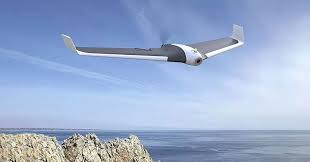
\includegraphics[width=0.65\textwidth]{imagenes/Dronalafija.jpeg}\\[0.5ex]
    {\small \textbf{Figura \thefigure.} Dron de ala fija. Fuente: \cite{DronFija}.}
    \addcontentsline{lof}{figure}{\protect\numberline{\thefigure}Dron de ala fija}
    \end{center}

    \item \textbf{Multirrotores (\textit{Multi-rotors}).} Constituyen la plataforma de referencia para este Trabajo de Fin de Grado. Su configuración, habitualmente basada en cuatro motores, permite un control directo. Su capacidad de despegue y aterrizaje vertical (VTOL), junto con su elevada agilidad, resulta esencial para mantener a un objetivo móvil dentro del campo de visión de la cámara de forma continua. La Figura \ref{fig:dron-multirrotor} presenta un ejemplo de esta configuración.

     \begin{center}
    \refstepcounter{figure}\label{fig:dron-multirrotor}
    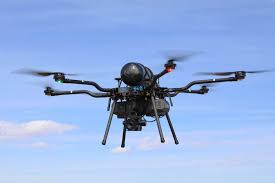
\includegraphics[width=0.65\textwidth]{imagenes/DronRotores.jpeg}\\[0.5ex]
    {\small \textbf{Figura \thefigure.} Dron multirrotor. Fuente: \cite{DronMotor}.}
    \addcontentsline{lof}{figure}{\protect\numberline{\thefigure}Dron multirrotor}
    \end{center}

    \item \textbf{Híbridos (VTOL \textit{Fixed-wing}).} Tratan de combinar la autonomía del ala fija con la versatilidad del multirrotor, aunque su mayor complejidad mecánica y de control suele traducirse en un incremento del peso, el coste y la dificultad de integración. La Figura \ref{fig:dron-vtol} presenta un ejemplo de plataforma VTOL de ala fija.

    \begin{center}
    \refstepcounter{figure}\label{fig:dron-vtol}
    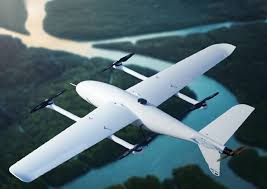
\includegraphics[width=0.65\textwidth]{imagenes/DronVtol.jpeg}\\[0.5ex]
    {\small \textbf{Figura \thefigure.} Dron VTOL de ala fija. Fuente: \cite{DronVtol}.}
    \addcontentsline{lof}{figure}{\protect\numberline{\thefigure}Dron VTOL de ala fija}
    \end{center}
\end{itemize}

\subsection{Aplicaciones actuales}


Entre sus distintas configuraciones, el dron multirrotor se ha consolidado como la plataforma más extendida debido a su maniobrabilidad, su facilidad de despliegue y su capacidad de vuelo estacionario, cualidades especialmente valiosas en operaciones que requieren cercanía al entorno y una respuesta rápida ante cambios del escenario.

\vspace{0.4cm}

Tradicionalmente, muchas de estas operaciones han dependido de un control humano directo, en el que un operador supervisa la trayectoria, corrige desviaciones y decide cada maniobra relevante. Este enfoque puede resultar suficiente en escenarios simples o muy controlados; sin embargo, pierde eficacia cuando el entorno es dinámico, cuando aparecen obstáculos imprevistos o cuando el objetivo modifica su trayectoria de forma continua.

\vspace{0.4cm}

En este contexto, la navegación autónoma surge como una solución tecnológica necesaria no solo para mejorar el rendimiento del sistema, sino también para reducir la carga de trabajo del operador humano. En misiones prolongadas, repetitivas o de alta exigencia, la dependencia constante del pilotaje manual incrementa el riesgo de fatiga, errores de supervisión y pérdida de eficacia operativa. La incorporación de capacidades autónomas permite automatizar tareas como el seguimiento de trayectorias, la corrección del movimiento y la respuesta ante cambios del entorno, disminuyendo la intervención continua del operador. Además, este enfoque contribuye a optimizar recursos y a abaratar costes operativos, al reducir la necesidad de control manual permanente y favorecer misiones más estables, seguras y sostenibles en el tiempo.

\vspace{0.4cm}

A partir de esta idea, la navegación autónoma adquiere especial relevancia en varias situaciones de uso:

\vspace{0.4cm}

\noindent\textbf{Utilización en agricultura:} En el ámbito de la agricultura de precisión, la navegación autónoma permite recorrer parcelas extensas, mantener trayectorias estables y adaptar el vuelo a las características del terreno o del cultivo \cite{WebDronAgri}. Esto facilita tareas como la supervisión del estado de las plantaciones, la detección de incidencias y la recopilación sistemática de información, reduciendo al mismo tiempo la intervención manual continua del operador.

  \begin{center}
    \refstepcounter{figure}\label{fig:dron-Cultivos}
    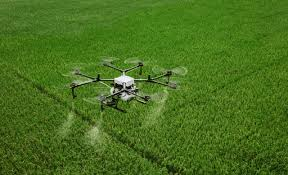
\includegraphics[width=0.65\textwidth]{imagenes/DronRegando.jpeg}\\[0.5ex]
    {\small \textbf{Figura \thefigure.} Dron utilizado en agricultura. Fuente: \cite{ImagenDronRegando}.}
    \addcontentsline{lof}{figure}{\protect\numberline{\thefigure}Dron monitoreando cultivos}
    \end{center}

\vspace{0.3cm}

\noindent\textbf{Apoyo en emergencias y búsqueda de objetivos:} En escenarios de emergencia, catástrofe o difícil acceso, la navegación autónoma permite explorar áreas amplias, evitar obstáculos y centrar la misión en la localización de objetivos de interés, como personas, embarcaciones, vehículos o puntos críticos del terreno. Esta capacidad resulta  valiosa en operaciones de apoyo en emergencias, donde el sistema debe reaccionar, adaptarse a cambios del entorno y mantener una búsqueda continua \cite{WebDronRescate}.

 \begin{center}
    \refstepcounter{figure}\label{fig:dron-Rescate}
    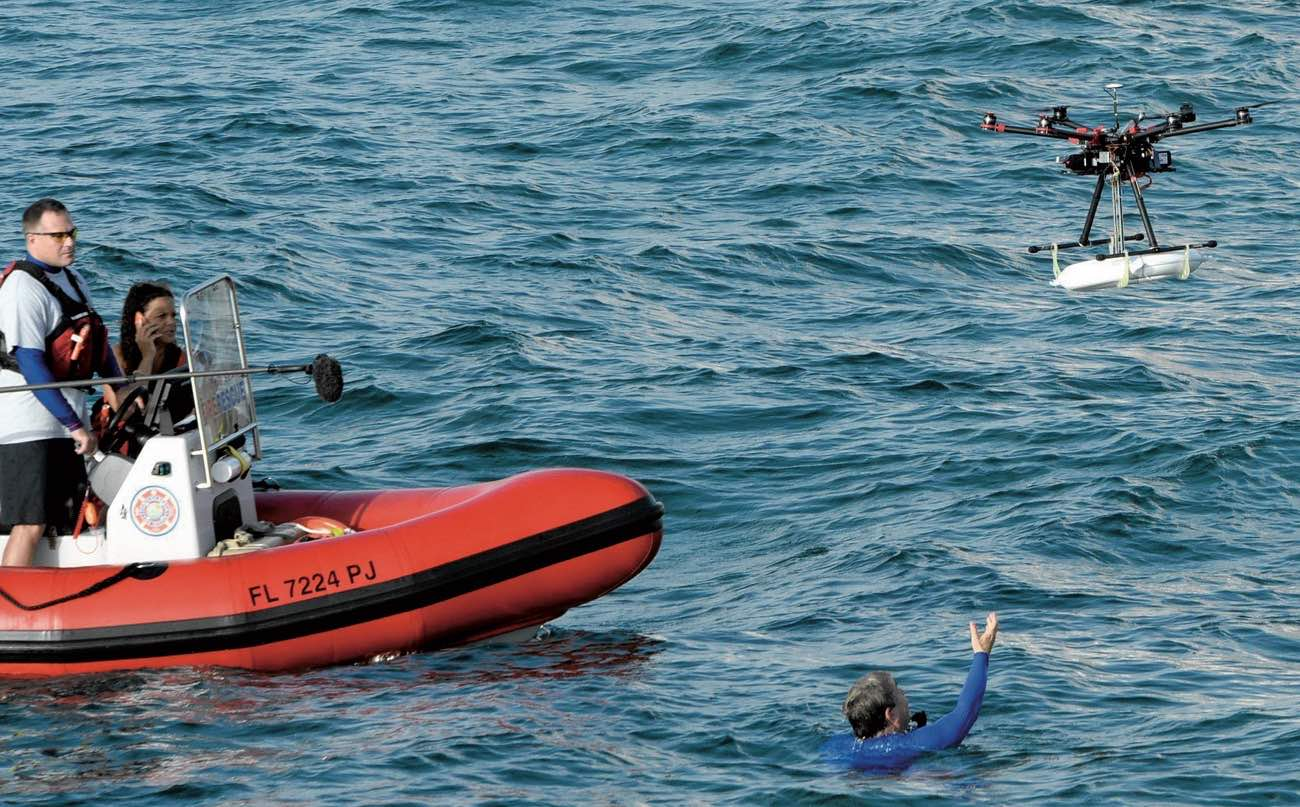
\includegraphics[width=0.65\textwidth]{imagenes/DronRescate.jpeg}\\[0.5ex]
    {\small \textbf{Figura \thefigure.} Dron utilizado en busqueda y rescate Marítimo. Fuente: \cite{ImagenDronRescate}.}
    \addcontentsline{lof}{figure}{\protect\numberline{\thefigure}Dron utilizado en Busqueda y rescate Marítimo}
  \end{center}


\vspace{0.4cm}

\noindent\textbf{Transporte autónomo de mercancías:} En entornos urbanos, industriales o logísticos \cite{WebDronMerca}, los UAV pueden convertirse en una alternativa eficiente para el envío de pequeñas cargas, repuestos o material de primera necesidad. En este tipo de operaciones, la navegación autónoma permite reajustar la ruta ante restricciones del entorno, variaciones en el trayecto o condiciones externas no previstas, manteniendo al mismo tiempo un vuelo estable y seguro .

\vspace{0.2cm}
    \begin{center}
      \refstepcounter{figure}\label{fig:dron-Transporte}
      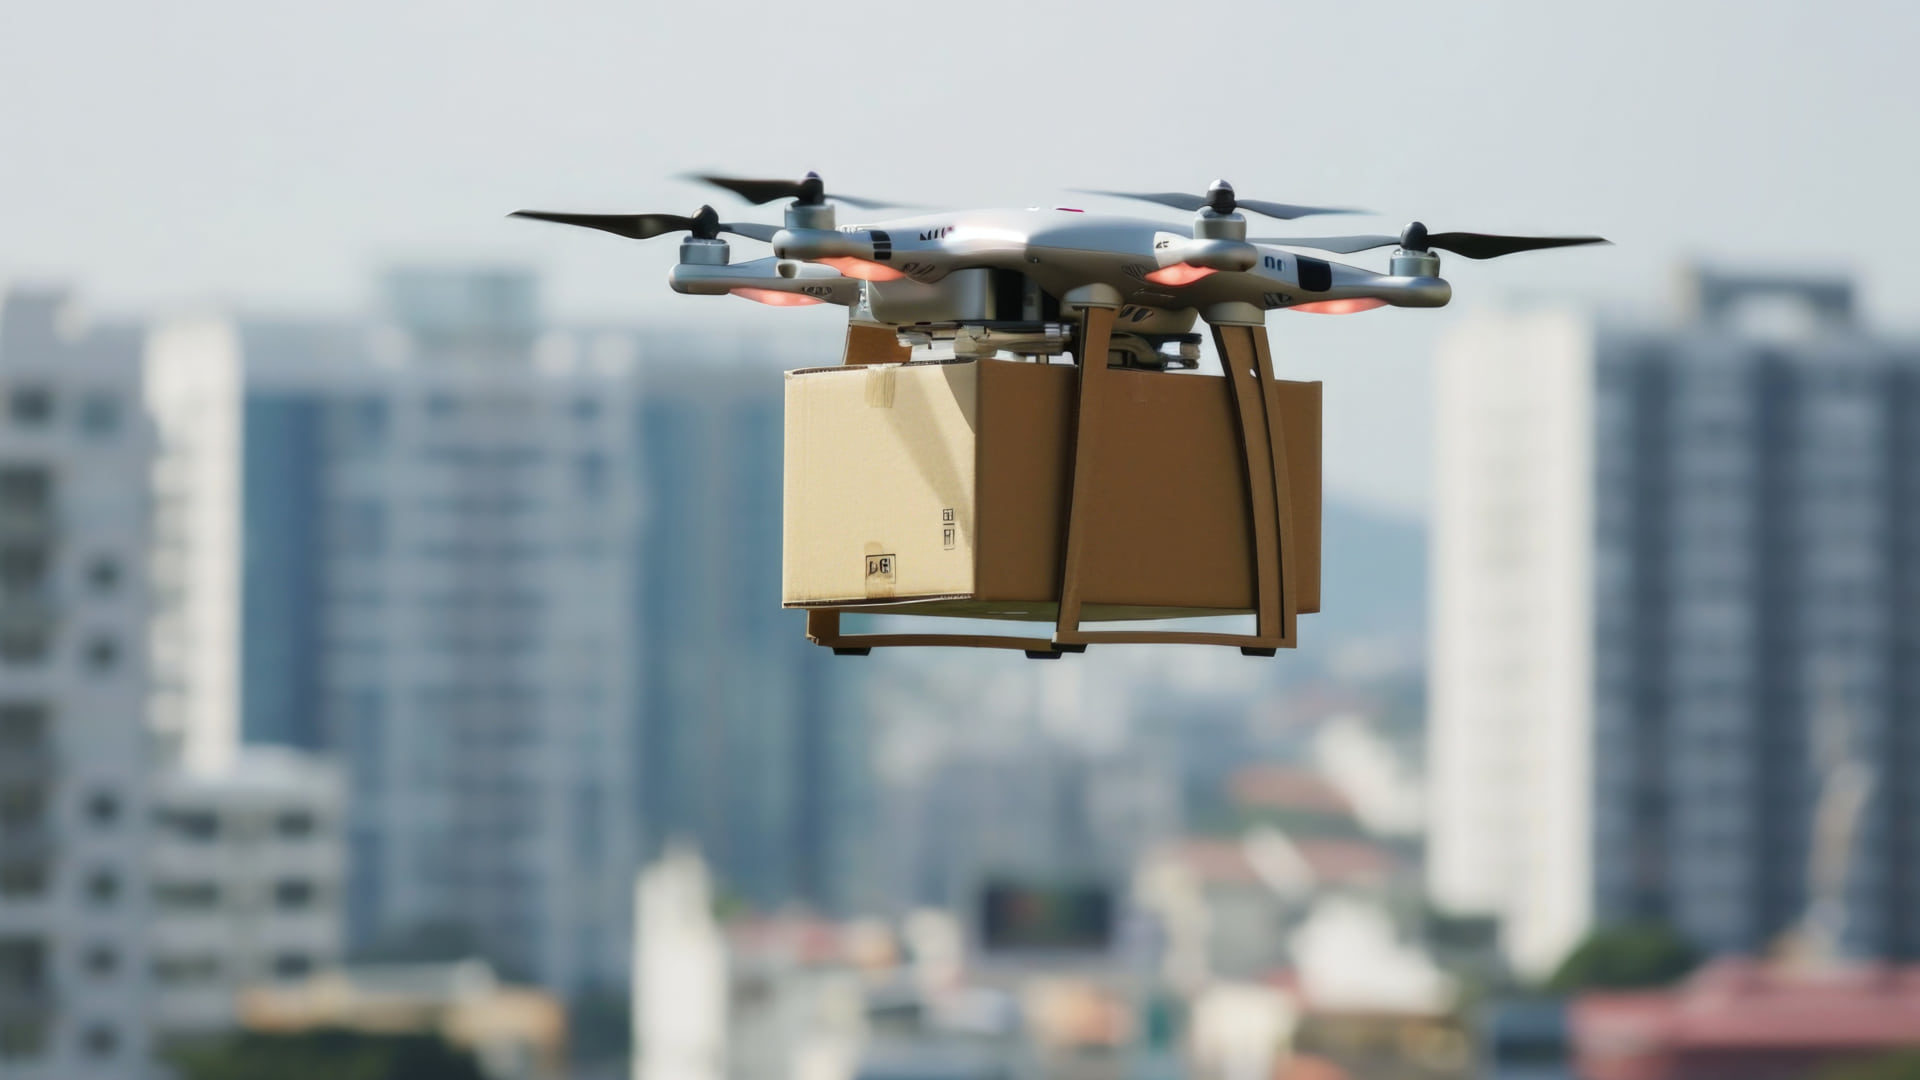
\includegraphics[width=0.65\textwidth]{imagenes/DronMerca.jpg}\\[0.5ex]
      {\small \textbf{Figura \thefigure.} Dron utilizado para transporte de paquetes. Fuente: \cite{ImagenDronMerca}.}
      \addcontentsline{lof}{figure}{\protect\numberline{\thefigure}Dron utilizado transporte de paquetes}
    \end{center}


\vspace{0.4cm}

\noindent\textbf{Operaciones militares y de defensa:} Este es el caso de uso más próximo al enfoque de este Trabajo de Fin de Grado. En misiones de reconocimiento, vigilancia, defensa, intercepción \cite{chavez2024emulating, WebDronDefensa} y seguimiento de UAV enemigos, la capacidad de reaccionar ante amenazas dinámicas resulta fundamental. En estos escenarios, el sistema no solo debe desplazarse, sino también detectar, seguir y mantener el objetivo dentro del campo de visión, corrigiendo su trayectoria en tiempo real incluso ante maniobras evasivas.

\vspace{0.2cm}

 \begin{center}
      \refstepcounter{figure}\label{fig:dron-Defensa}
      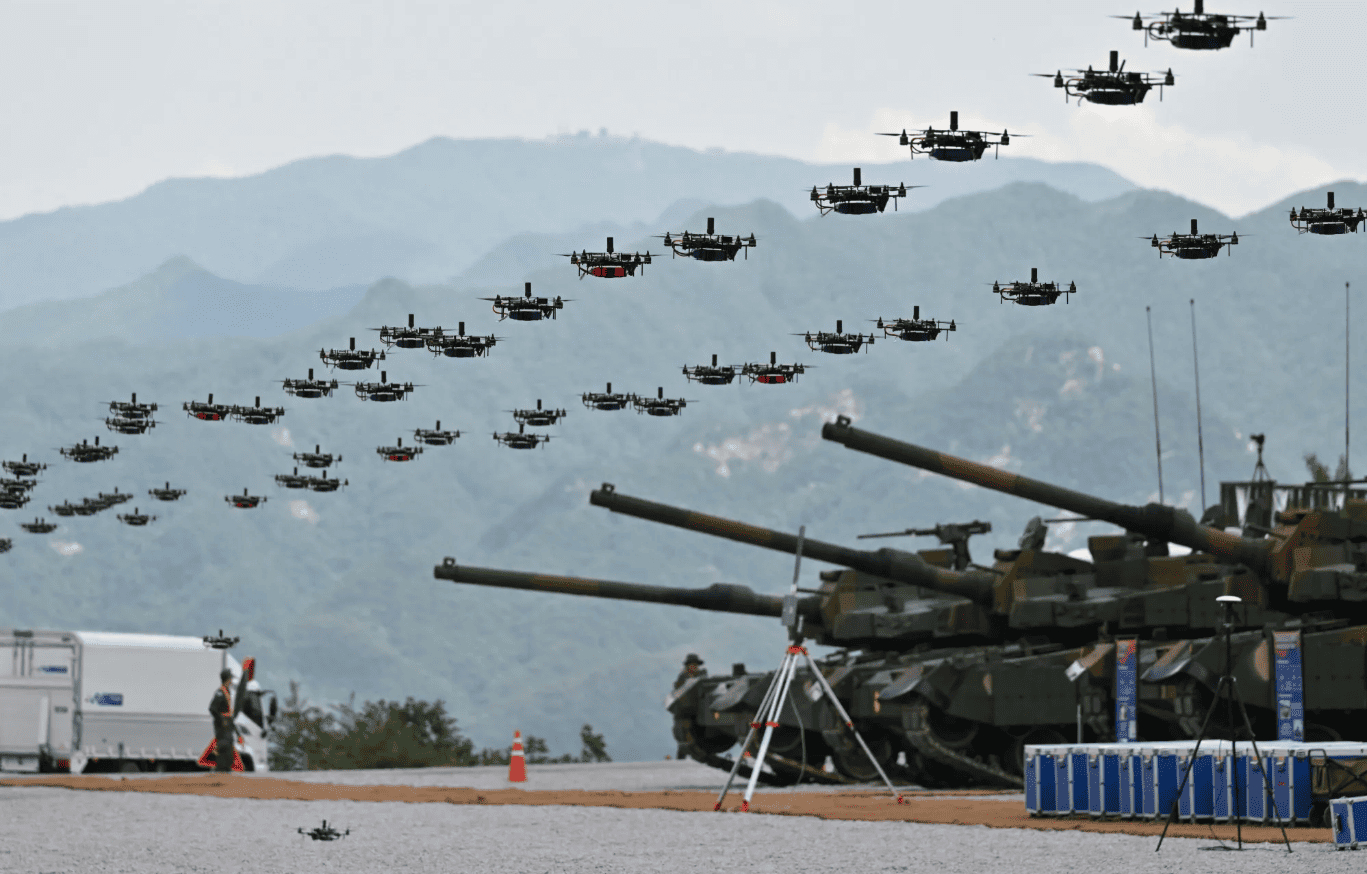
\includegraphics[width=0.65\textwidth]{imagenes/DronDefensa.jpeg}\\[0.5ex]
      {\small \textbf{Figura \thefigure.} Drones utilizados para operaciones militares. Fuente: \cite{ImagenDronDefensa}.}
      \addcontentsline{lof}{figure}{\protect\numberline{\thefigure} Drones utilizados para operaciones militares}
    \end{center}

\vspace{1cm}

En consecuencia, los métodos basados exclusivamente en pilotaje humano o en trayectorias rígidamente prefijadas resultan insuficientes cuando el sistema debe desenvolverse en entornos no estructurados y frente a objetivos dinámicos. Además, este enfoque incrementa la dependencia de pilotos con un alto nivel de entrenamiento, capaces de mantener decisiones rápidas y precisas durante situaciones de elevada exigencia operativa. Por ello, este Trabajo de Fin de Grado se orienta hacia estrategias de percepción visual y control de navegación que permitan reducir esa dependencia, automatizar tareas críticas de seguimiento e intercepción y dotar al UAV cazador de una respuesta robusta, precisa y adaptable en tiempo real.

\vspace{0.4cm}


\section{ Métodos de Control de Navegación para UAVs}

Para alcanzar este nivel de autonomía, el control del vehículo no puede entenderse como una acción aislada, sino como parte de un sistema integrado de Guiado, Navegación y Control, habitualmente denominado GNC (\textit{Guidance, Navigation and Control}). Este marco organiza el comportamiento inteligente de la aeronave en tres niveles jerárquicos y complementarios: el guiado determina la estrategia de la misión y la trayectoria a seguir; la navegación estima el estado del UAV y su posición relativa respecto al entorno; y el control transforma esta información en comandos específicos de actitud y empuje. En conjunto, el sistema GNC permite cerrar el lazo entre la percepción sensorial y la respuesta dinámica del dron, un factor crítico cuando el escenario de operación cambia en tiempo real y el objetivo se mueve de forma continua .

\vspace{0.3cm}

Dentro de este esquema, el control de navegación actúa como el núcleo de decisión táctica. Su función principal es procesar la información proveniente del módulo de navegación para generar comandos de movimiento que permitan cumplir objetivos complejos, como la persecución de una presa. En este tipo de misiones, el éxito no depende únicamente de una detección correcta, sino de la capacidad del algoritmo para orquestar un movimiento fluido que mantenga al objetivo dentro del campo de visión sin comprometer la estabilidad del vuelo.

\vspace{0.3cm}

Dada la complejidad de este desafío, la literatura científica ha evolucionado hacia diversos paradigmas de control, diferenciados principalmente por la fuente de los datos y la arquitectura del procesamiento \ref{fig:esquema-Sevoing}. Estos enfoques se pueden clasificar en tres grandes categorías : los métodos basados en localización global, los enfoques fundamentados en aprendizaje profundo (\textit{Deep Learning}) y los sistemas de control basado en imagen (\textit{Visual Servoing}). Cada una de estas metodologías presenta un compromiso distinto entre precisión, coste computacional y robustez, factores que determinan su idoneidad para operar en sistemas empotrados de recursos limitados. A continuación, se describen los fundamentos y aplicaciones de estos paradigmas para situar las soluciones propuestas en la literatura y preparar el marco metodológico del trabajo.


\begin{center}
      \refstepcounter{figure}\label{fig:esquema-Sevoing}
      
      % Aquí aplicamos el truco de la caja (\makebox) y el tamaño 1.4
      \makebox[\textwidth][c]{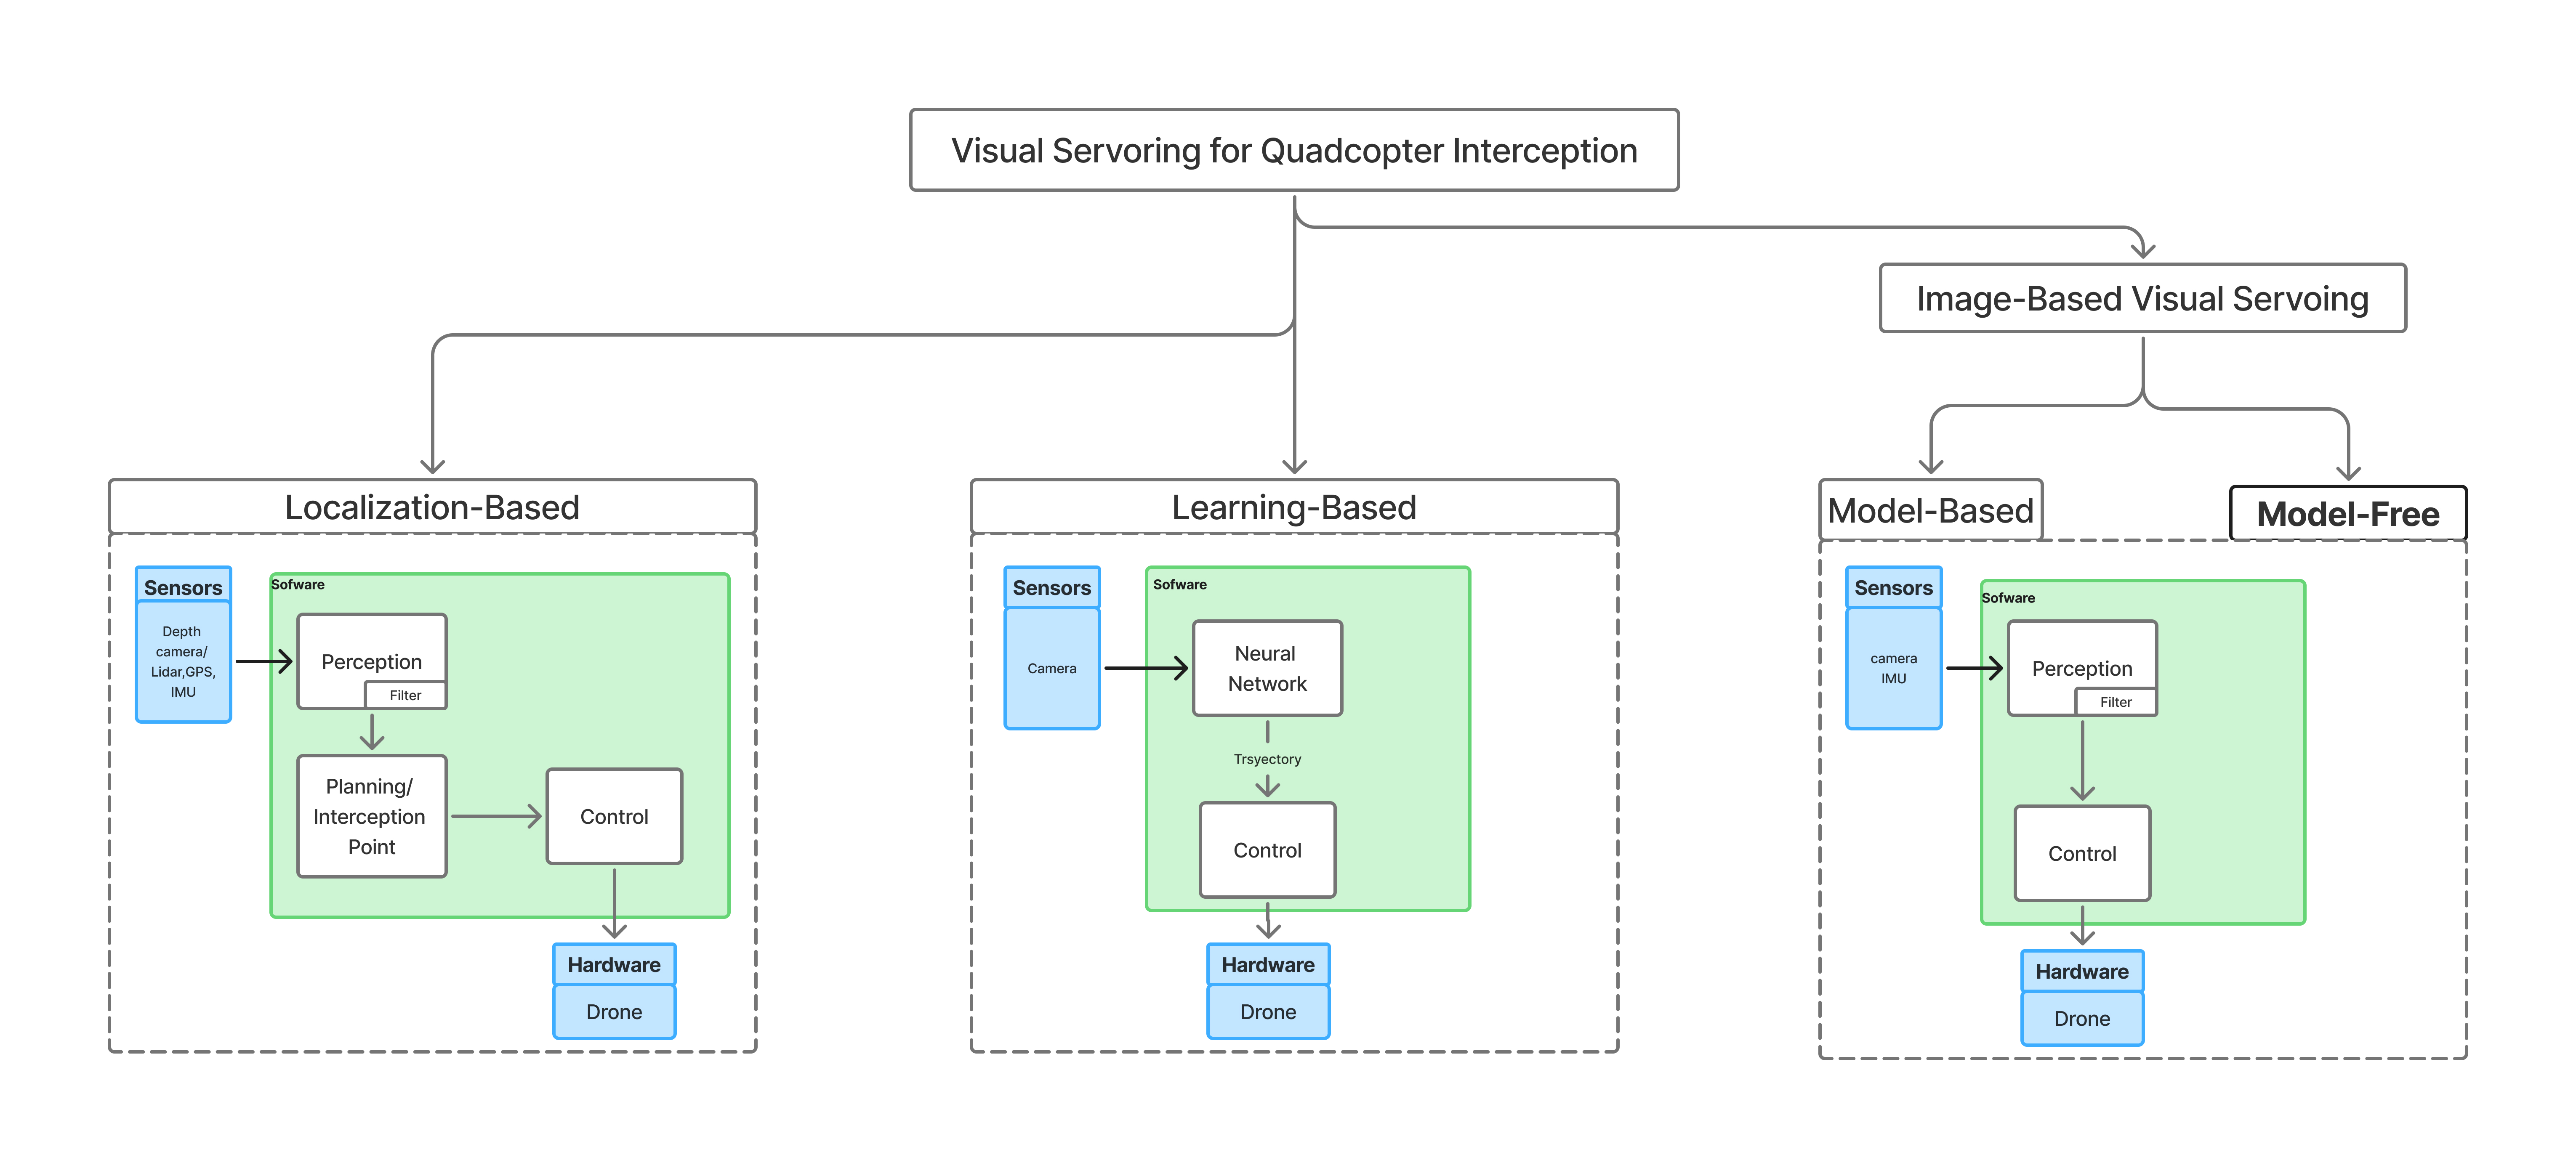
\includegraphics[width=1.4\textwidth]{imagenes/TipoControles2.jpg}}\\[0.5ex]
      
      {\small \textbf{Figura \thefigure.} Diferencias entre los tipos de algoritmos de visual Servoing(Elaboración propia).}
      \addcontentsline{lof}{figure}{\protect\numberline{\thefigure} Tipos de algoritmos de visual Servoing (Elaboración propia)}
\end{center}

\subsection{Tipos de control de navegación}




Los \textbf{métodos basados en localización}, encuadrados habitualmente en el paradigma \textit{Position-Based Visual Servoing} (PBVS), tienen como objetivo reconstruir la posición y la orientación del blanco en el espacio cartesiano a partir de la información visual \cite{chaumette2006visual}. Esta estimación tridimensional permite definir trayectorias de intercepción con un mayor grado de precisión, algo especialmente útil en misiones de seguimiento e intercepción con cuadricópteros. Dentro de esta familia, algunos trabajos recurren a controladores predictivos no lineales que optimizan la acción de control en un horizonte temporal, teniendo en cuenta tanto la evolución prevista del objetivo como las restricciones dinámicas del UAV. Otros enfoques emplean lazos de control sobre velocidades angulares para hacer coincidir la línea de visión con el vector de velocidad del vehículo, o modelan la trayectoria del blanco en tres dimensiones para escoger puntos de interceptación más convenientes. De igual modo, también se han propuesto arquitecturas de doble lazo PID que aprovechan los estados tridimensionales estimados del objetivo para seguir blancos terrestres o aéreos\cite{rodriguezRamos2021autonomous}.

\vspace{0.3cm}

En definitiva, la principal fortaleza de PBVS radica en su capacidad para prever el movimiento del objetivo y determinar puntos de interceptación. No obstante, su rendimiento queda condicionado por una estimación fiable de la profundidad y por una calibración rigurosa de la cámara. Asimismo, una parte importante de los trabajos revisados complementa la información visual con sensores adicionales, como radares o cámaras estéreo y de profundidad, con el fin de mejorar la reconstrucción espacial y aumentar la robustez del sistema.

\vspace{0.3cm}

Los \textbf{métodos basados en aprendizaje} delegan una parte importante del control en modelos entrenados con datos, normalmente redes neuronales capaces de inferir comandos de navegación de forma directa a partir de la información visual. Dentro de esta familia destacan enfoques de aprendizaje supervisado y, especialmente, técnicas de aprendizaje por refuerzo, que han mostrado una notable capacidad de adaptación frente al ruido sensorial y ante entornos dinámicos o poco estructurados. Esta flexibilidad resulta especialmente atractiva en tareas de intercepción, donde el dron debe reaccionar en tiempo real a cambios imprevistos de la escena o de la trayectoria del objetivo \cite{weber2025autonomous, katkuri2024uav}. No obstante, su aplicación práctica sigue presentando dificultades relevantes: requieren grandes volúmenes de datos y tiempos de entrenamiento elevados, suelen quedar condicionados por los escenarios utilizados durante el aprendizaje y continúan arrastrando problemas importantes de transferencia entre simulación y mundo real. A ello se suma la cuestión de la generalización, ya que un modelo entrenado en condiciones concretas puede perder fiabilidad cuando cambian el entorno, la dinámica del vehículo o las perturbaciones externas \cite{guazzaloca2025learning}.

\vspace{0.3cm}

Por su parte, los \textbf{métodos basados en imagen}, agrupados bajo el paradigma \textit{Image-Based Visual Servoing} (IBVS), utilizan directamente el error medido en el plano imagen para generar la acción de control. En lugar de reconstruir por completo la geometría tridimensional del objetivo, estos enfoques trabajan con características visuales como el desplazamiento del blanco respecto al centro de la imagen o la variación de su tamaño aparente. Esta decisión reduce la dependencia respecto a estimaciones geométricas completas y suele favorecer soluciones más ligeras y mejor adaptadas a plataformas embarcadas con recursos limitados \cite{chaumette2006visual, yang2024high, yan2024precise}.



\vspace{0.3cm}

\subsection{Conceptos de Visual Servoing (IBVS)}

Dentro de IBVS pueden distinguirse, a su vez, dos enfoques. El primero corresponde a los métodos basados en modelo, que incorporan de forma explícita la dinámica del cuadricóptero y la cinemática visual en el diseño del controlador. Estos métodos permiten respuestas más predictivas, un seguimiento más preciso y, en algunos casos, garantías formales de estabilidad, pero a cambio requieren un modelado más detallado del sistema y un mayor esfuerzo de ajuste \cite{asl2014adaptive, yang2024high, yan2024precise}. El segundo enfoque es el de los métodos libres de modelo, en los que el controlador abstrae gran parte de la dinámica interna del UAV y delega la estabilización básica en el autopiloto o en los lazos de bajo nivel ya disponibles. Esta aproximación reduce la carga computacional y simplifica la integración práctica, aunque puede ofrecer una menor capacidad de respuesta ante maniobras extremadamente agresivas o escenarios muy exigentes \cite{wyder2019autonomous, lee2023air, vanDerAa2024ibvs}.

\vspace{0.3cm}

Por tanto, la elección entre PBVS, enfoques basados en aprendizaje e IBVS no depende únicamente de cuál resulte más sofisticado desde un punto de vista teórico, sino de cuál se adapta mejor al contexto de aplicación. PBVS aporta una representación espacial rica, pero exige una percepción 3D precisa; los métodos basados en aprendizaje ofrecen flexibilidad, aunque todavía presentan dificultades importantes de entrenamiento y transferencia al entorno real; e IBVS proporciona una relación especialmente favorable entre simplicidad, latencia y viabilidad en tiempo real. En problemas donde la percepción ya suministra detecciones en el plano imagen, los enfoques IBVS libres de modelo constituyen una opción especialmente coherente, ya que permiten conectar de forma directa la localización visual del objetivo con la generación de consignas de control sin introducir una complejidad geométrica o computacional excesiva. Esta observación explica que buena parte de la literatura combine percepción visual, estimación ligera y control reactivo, y sirve además como punto de partida para la metodología desarrollada posteriormente.



\section{Deep Learning}

El \textit{Deep Learning} es una rama del aprendizaje automático basada en redes neuronales artificiales con múltiples capas, capaces de aprender representaciones jerárquicas directamente a partir de los datos. A diferencia de otros enfoques más tradicionales, reduce la necesidad de diseñar manualmente las características de entrada, ya que el propio modelo ajusta internamente niveles sucesivos de abstracción durante el proceso de entrenamiento \cite{goodfellow2016deep}.

\vspace{0.3cm}

El desarrollo de esta disciplina ha estado impulsado por la disponibilidad de grandes volúmenes de datos, el aumento de la capacidad de cómputo y la mejora de los métodos de entrenamiento. Gracias a ello, el \textit{Deep Learning} se ha consolidado como un enfoque general para abordar tareas de clasificación, regresión, predicción y generación de datos en contextos muy diversos. Esta flexibilidad explica su relevancia dentro del aprendizaje automático actual y justifica su presencia como base conceptual en numerosos sistemas inteligentes \cite{goodfellow2016deep}.



\begin{center}
      \refstepcounter{figure}\label{fig:red-neuronal-multicapa}
      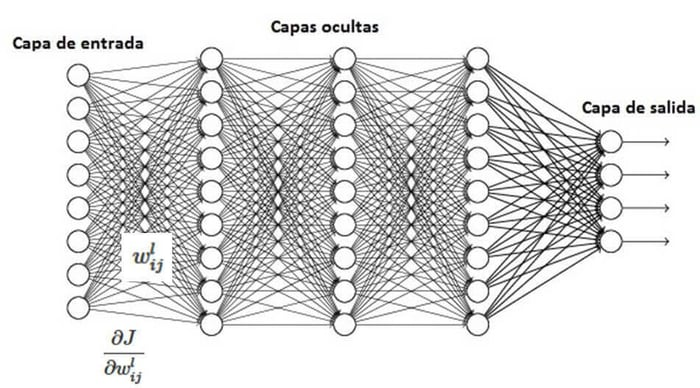
\includegraphics[width=0.82\textwidth]{imagenes/capasRed.jpg}\\[0.5ex]
      {\small \textbf{Figura \thefigure.} Esquema general de una red neuronal multicapa. Fuente: \cite{stalearning2018gradiente}.}
      \addcontentsline{lof}{figure}{\protect\numberline{\thefigure}Esquema general de una red neuronal multicapa}
\end{center}



\vspace{0.3cm}

\section{Visión por Computador}

La visión por computador, también conocida como visión artificial o visión computarizada, es una rama de la inteligencia artificial que agrupa técnicas y herramientas orientadas a adquirir, procesar e interpretar información visual procedente del entorno. A partir de imágenes o secuencias de vídeo, estos sistemas pueden extraer características relevantes que facilitan la detección, la clasificación y el análisis de objetos, escenas y movimientos.

\vspace{0.3cm}

Este campo integra conocimientos de procesamiento digital de imágenes, estadística, aprendizaje automático y robótica con el propósito de desarrollar sistemas capaces de comprender el contenido visual y actuar a partir de él, de forma autónoma o asistida. En este sentido, la visión por computador busca dotar a las máquinas de capacidades de percepción útiles para interpretar su entorno y apoyar procesos posteriores de decisión y control.

\vspace{0.3cm}

Sus orígenes suelen situarse en la década de 1960, cuando comenzaron a explorarse métodos para que los ordenadores reconocieran formas sencillas en imágenes bidimensionales. En aquella etapa inicial, las aplicaciones se centraban en tareas relativamente básicas, como la detección de bordes o el reconocimiento de patrones geométricos, debido tanto a las limitaciones del hardware disponible como a la escasez de datos con los que entrenar y validar los modelos.

\vspace{0.3cm}

En las últimas décadas, el incremento de la capacidad de cómputo, la disponibilidad de grandes conjuntos de datos y el desarrollo de arquitecturas basadas en redes neuronales convolucionales (CNN) han impulsado notablemente la evolución del área. Gracias a ello, hoy es posible abordar tareas complejas como la detección de objetos en tiempo real, la segmentación semántica, el reconocimiento facial o el seguimiento automático, y han surgido detectores especialmente influyentes como Faster R-CNN y la familia YOLO \cite{FunRcnn}.

\vspace{0.3cm}

Entre sus aplicaciones destacan la conducción autónoma, la videovigilancia, la robótica, la inspección automática y la interacción persona-máquina. En el contexto de este trabajo, la visión por computador se empleará como base perceptiva para la detección y el seguimiento visual del dron objetivo, lo que enlaza de forma natural con la detección de objetos tratada en el apartado siguiente .

\vspace{0.3cm}

\subsection{Paradigmas de detección de objetos}

El objetivo fundamental de la detección de objetos consiste en localizar y clasificar regiones de interés dentro de una imagen, normalmente representadas mediante cajas delimitadoras. La detección debe resolver simultáneamente qué objetos aparecen y dónde se encuentran. Por ello, se trata de un problema más exigente desde el punto de vista computacional y metodológico, ya que combina percepción semántica y localización espacial en una misma tarea.

\begin{center}
\refstepcounter{figure}\label{fig:detecion-objetos-ejemplo}
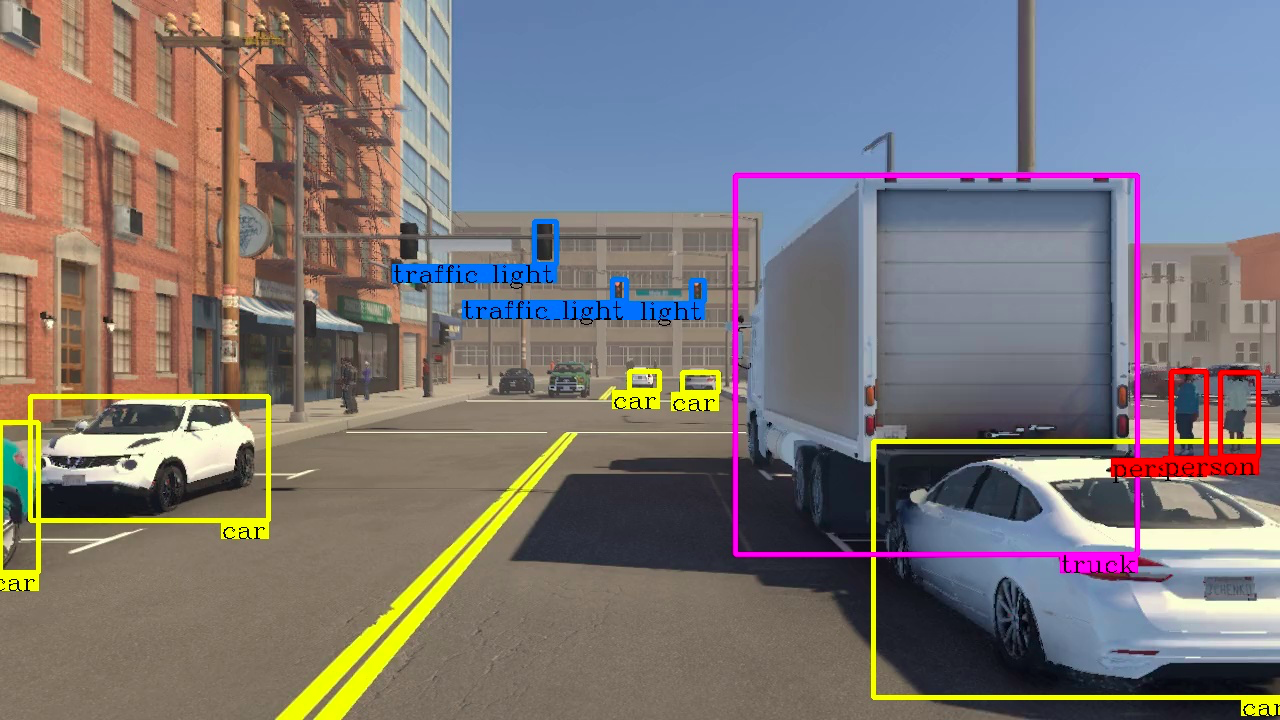
\includegraphics[width=0.78\textwidth]{imagenes/detecionObj.png}\\[0.5ex]
{\small \textbf{Figura \thefigure.} Ejemplo ilustrativo de detección de objetos mediante cajas delimitadoras. Fuente: \cite{innovatiana2024objectdetection}.}
\addcontentsline{lof}{figure}{\protect\numberline{\thefigure}Ejemplo ilustrativo de detección de objetos mediante cajas delimitadoras}
\end{center}
\vspace{0.3cm}

Antes de la consolidación de los enfoques basados en redes profundas, una parte importante de los métodos de detección se apoyaba en estrategias de ventana deslizante. En ese marco, modelos como \textit{Deformable Parts Model} (DPM) recorrían la imagen evaluando un gran número de subregiones candidatas, lo que permitía detectar objetos a distintas escalas y posiciones, pero a costa de una carga computacional muy elevada. Aunque estos enfoques marcaron una etapa importante en la evolución de la detección de objetos, su coste de inferencia y su limitada capacidad de adaptación a escenas complejas hicieron evidente la necesidad de arquitecturas más eficientes \cite{felzenszwalb2010dpm}.

\vspace{0.3cm}

La transición hacia el \textit{Deep Learning} se consolidó con la familia R-CNN, que introdujo un esquema de dos etapas. En su formulación original, R-CNN generaba primero un conjunto de regiones potencialmente relevantes mediante búsqueda selectiva, después extraía características con una red convolucional para cada una de esas regiones y, finalmente, realizaba la clasificación. Este planteamiento supuso un avance decisivo en precisión, pero seguía penalizado por el hecho de procesar cada región de manera separada y por depender de un mecanismo externo de propuesta de regiones. Faster R-CNN mejoró este pipeline al integrar la generación de propuestas dentro de la propia red mediante una \textit{Region Proposal Network} (RPN). Con ello, el sistema gana coherencia y velocidad respecto a R-CNN, aunque sigue siendo un detector de dos etapas y, por tanto, mantiene una latencia relativamente mayor que otras alternativas \cite{FunRcnn, diffTwoStage}.

\vspace{0.3cm}
\begin{center}
    \refstepcounter{figure}\label{fig:FunRccnn}
    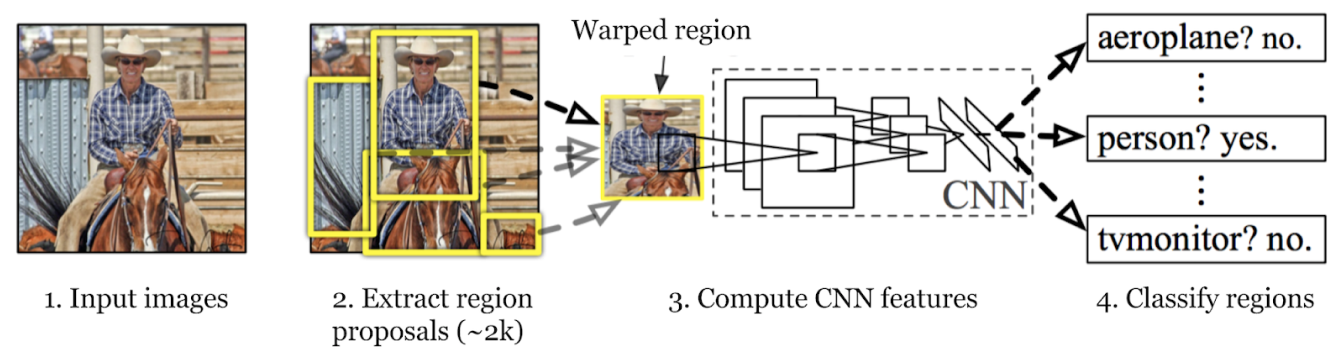
\includegraphics[width=0.65\textwidth]{imagenes/FunRcnn.png}\\[0.5ex]
    {\small \textbf{Figura \thefigure.} Esquema simplificado del funcionamiento de R-CNN, \cite{FunRcnn}.}
    \addcontentsline{lof}{figure}{\protect\numberline{\thefigure}Esquema simplificado del funcionamiento de R-CNN}
\end{center}

\vspace{0.3cm}

Frente a esta familia de detectores, los métodos de una sola etapa reformulan la detección como un problema unificado de predicción directa. En lugar de separar explícitamente la propuesta de regiones y la clasificación, una única red procesa la imagen completa y estima de forma simultánea las categorías, las puntuaciones de confianza y las coordenadas de las cajas delimitadoras. Esta simplificación reduce la complejidad del pipeline y favorece tiempos de inferencia mucho menores, una propiedad especialmente relevante en plataformas embarcadas y en escenarios dinámicos como la intercepción aire-aire, donde la frecuencia de actualización del detector resulta tan importante como su precisión.

\vspace{0.3cm}

\subsection{YOLO}

La familia YOLO (\textit{You Only Look Once}) constituye el ejemplo más influyente de detector de una sola etapa basado en regresión unificada. Su aportación principal consiste en reformular la detección de objetos como un problema de predicción directa sobre la imagen completa, evitando la separación explícita entre propuesta de regiones y clasificación. De este modo, la red estima de forma conjunta la localización de las cajas delimitadoras y la probabilidad de las clases presentes en la escena.
\vspace{0.3cm}


Desde un punto de vista operativo, estos detectores combinan tres ideas fundamentales: una partición implícita de la escena en regiones de predicción, la estimación directa de cajas delimitadoras y puntuaciones de confianza mediante regresión, y una etapa final de depuración basada en métricas de solapamiento como la intersección sobre unión (IoU) y en procedimientos como \textit{Non-Maximum Suppression} (NMS). Esta formulación permite generar detecciones con latencias reducidas y con una frecuencia de actualización compatible con aplicaciones de tiempo real.

\vspace{0.3cm}


\begin{center}
    \refstepcounter{figure}\label{fig:yolo-funcionamiento}
    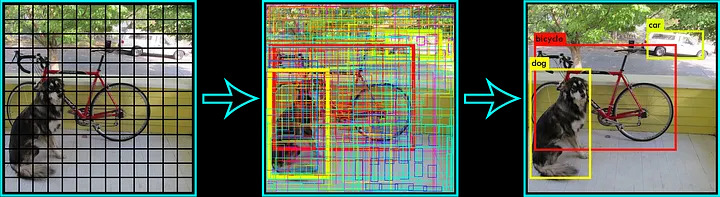
\includegraphics[width=0.65\textwidth]{imagenes/yolo-esquema.jpeg}\\[0.5ex]
    {\small \textbf{Figura \thefigure.} Esquema simplificado del funcionamiento de Yolo, \cite{aiknow2024yolo}.}
    \addcontentsline{lof}{figure}{\protect\numberline{\thefigure}Esquema simplificado del funcionamiento de Yolo}
\end{center}

\vspace{0.3cm}

La literatura reciente ha consolidado a YOLO como una de las familias más extendidas en visión embarcada gracias a su equilibrio entre precisión, velocidad y facilidad de despliegue. En problemas de detección aérea, seguimiento e intercepción, este compromiso resulta especialmente valioso porque la utilidad del detector depende no solo de su exactitud espacial, sino también de su capacidad para suministrar observaciones consistentes a alta frecuencia. Además, al predecir directamente magnitudes continuas asociadas a la localización del blanco, estos modelos proporcionan una base adecuada para etapas posteriores de seguimiento visual, estimación geométrica e inferencia de distancia relativa \cite{terven2023comprehensive}.

\vspace{0.3cm}
\section{Geometría Proyectiva}

\vspace{0.3cm}
Una vez presentadas las técnicas de percepción visual y detección de objetos, resulta necesario introducir el marco geométrico que permite interpretar esa información en términos espaciales y relacionarla con el movimiento del dron. En este contexto, la geometría proyectiva constituye la base teórica que conecta los puntos del espacio tridimensional con su representación en el plano imagen. En navegación visual, esta disciplina resulta esencial porque la cámara no proporciona directamente una posición 3D del objetivo, sino una proyección bidimensional condicionada por la perspectiva, la orientación de la cámara y sus parámetros internos \cite{CameraModels, uvaPinholeCamera, bergamasco2019pinhole}. Antes de introducir el modelo geométrico de la cámara, conviene partir de la cámara estenopeica o modelo \textit{pinhole}, ya que constituye la aproximación más simple y utilizada para explicar cómo se forma una imagen.

\vspace{0.3cm}

\subsection{Cámara estenopeica}

La cámara estenopeica, también conocida como modelo \textit{pinhole}, es una idealización geométrica utilizada para describir cómo se forma una imagen a partir de la luz procedente del entorno. En este modelo, los rayos luminosos atraviesan un único orificio y se proyectan sobre un plano imagen, lo que permite relacionar de forma sencilla el espacio tridimensional con su representación bidimensional.

\vspace{0.3cm}

Sus antecedentes históricos se asocian a la cámara oscura y a las primeras observaciones sobre la propagación rectilínea de la luz.  desde la Antigüedad se estudiaron fenómenos de proyección similares, y con el tiempo estos principios dieron lugar a dispositivos estenopeicos cada vez más elaborados, primero con fines de observación y más adelante también con aplicaciones fotográficas y didácticas \cite{wikipediaCamaraEstenopeica}.

\vspace{0.3cm}

Desde un punto de vista funcional, su funcionamiento se basa en que solo una pequeña fracción de la luz procedente de cada punto de la escena atraviesa el orificio, lo que genera una imagen invertida sobre el plano de proyección. Así, el sistema no mide directamente la profundidad ni las coordenadas espaciales del entorno, sino su proyección en la imagen. Esta idea resulta fundamental para comprender cómo la posición, el tamaño aparente y la perspectiva de los objetos quedan codificados visualmente .

\vspace{0.3cm}

Tradicionalmente, la cámara estenopeica se construía de forma muy simple, mediante una caja opaca, un pequeño estenopo y una superficie fotosensible, como papel o película fotográfica, por lo que las exposiciones solían ser largas y el control de entrada de luz era manual. En la actualidad, ese mismo principio puede aplicarse también sobre dispositivos con sensores digitales, como los CCD, y sigue utilizándose con fines educativos, artísticos y experimentales. De este modo, puede compararse una versión histórica basada en captura analógica con variantes modernas apoyadas en tecnología digital \cite{wikipediaCamaraEstenopeica}.

\vspace{0.3cm}

\begin{center}
\refstepcounter{figure}\label{fig:camara-estenopeica-funcionamiento}
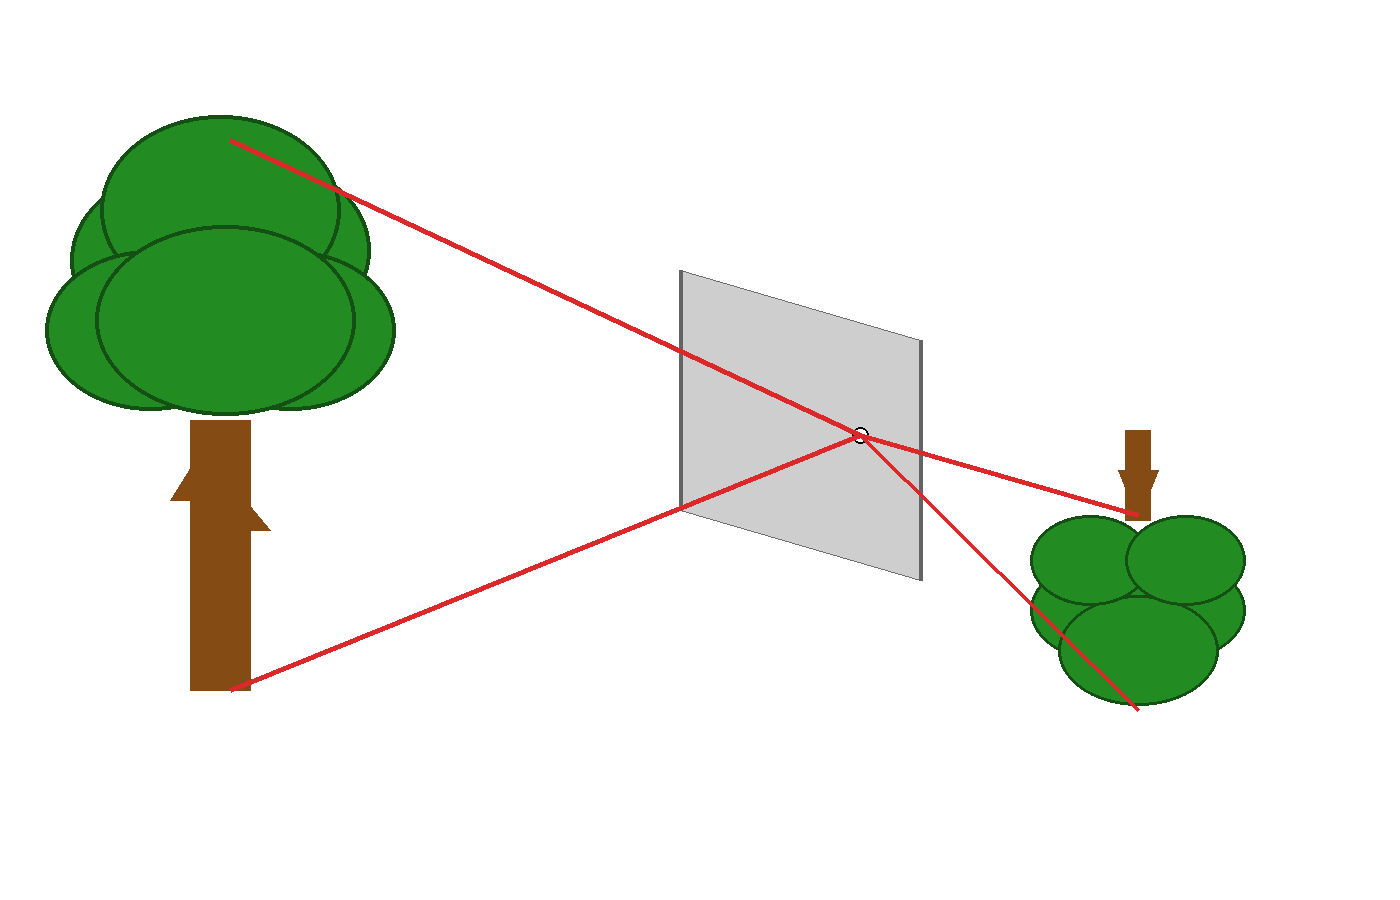
\includegraphics[width=0.78\textwidth]{imagenes/pinhole-camera-wikipedia-adaptada.png}\\[0.5ex]
{\small \textbf{Figura \thefigure.} Funcionamiento simplificado de una cámara estenopeica. Fuente: \cite{commonsPinholeCameraSvg}.}
\addcontentsline{lof}{figure}{\protect\numberline{\thefigure}Funcionamiento simplificado de una cámara estenopeica}
\end{center}

\vspace{0.3cm}

\subsection{Modelo geométrico de la cámara}

A partir de esta idealización, la proyección de un punto del mundo puede representarse de forma compacta mediante la relación entre parámetros extrínsecos, parámetros intrínsecos y coordenadas del punto observado. En forma homogénea, esta idea suele resumirse como:

\vspace{0.3cm}

\begin{equation}
s \left[\begin{array}{c}u \\ v \\ 1\end{array}\right] = K \cdot [R|t] \cdot \left[\begin{array}{c}X_w \\ Y_w \\ Z_w \\ 1\end{array}\right]
\end{equation}

\vspace{0.3cm}

donde la matriz intrínseca recoge parámetros como la distancia focal y el punto principal, mientras que la transformación extrínseca describe la posición y orientación de la cámara respecto al entorno. Aunque se trata de un modelo idealizado, resulta suficientemente expresivo para describir la mayor parte de los fenómenos geométricos relevantes en visión por computador \cite{opencvCalib3d}.

\vspace{0.3cm}

\begin{center}
\refstepcounter{figure}\label{fig:ibvs-esquema}
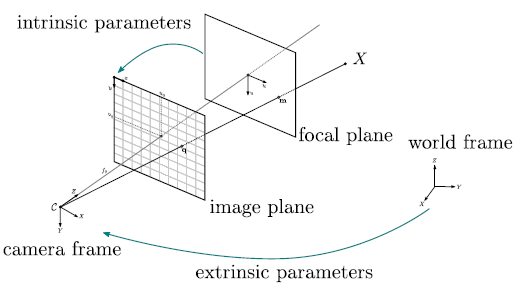
\includegraphics[width=0.65\textwidth]{imagenes/pinholeCamera2.jpeg}\\[0.5ex]
{\small \textbf{Figura \thefigure.} Esquema simplificado del modelo de cámara estenopeica. Fuente: \cite{openMVGCameras}.}
\addcontentsline{lof}{figure}{\protect\numberline{\thefigure}Esquema simplificado del modelo de cámara estenopeica}
\end{center}

\vspace{0.3cm}

\subsection{Usos en navegación visual}

En la literatura sobre \textit{visual servoing} y seguimiento de UAV, la geometría proyectiva se emplea principalmente con tres objetivos. En primer lugar, permite calibrar el sistema de visión y caracterizar propiedades como el campo de visión, el punto principal o las distorsiones introducidas por la óptica. En segundo lugar, proporciona la base para relacionar variables medidas en píxeles con magnitudes útiles para estimación y control, como la dirección de visión, la escala aparente del objetivo o su posición relativa. En tercer lugar, sirve de soporte para compensar el efecto de la actitud del vehículo y para diseñar controladores que actúan a partir del error visual observado \cite{asl2014adaptive, yang2024high}.

\vspace{0.3cm}

Por ello, incluso en enfoques IBVS que evitan una reconstrucción tridimensional completa, la geometría proyectiva sigue siendo una herramienta conceptual relevante. Más que un bloque aislado de reconstrucción 3D, actúa como un lenguaje común que conecta calibración, percepción y control dentro de los sistemas de navegación guiados por cámara \cite{vanDerAa2024ibvs}.

\vspace{0.3cm}
\section{Métodos de Control}

En robótica aérea, el control puede definirse como el conjunto de algoritmos encargados de manipular las variables de entrada del sistema, como la velocidad de los motores o las consignas de actitud, para lograr que las variables de salida del vehículo, entre ellas su posición, velocidad y orientación, sigan un comportamiento deseado. Su papel es fundamental para mantener la estabilidad frente a perturbaciones externas y para garantizar que el UAV cumpla de forma autónoma los objetivos de la misión .

\vspace{0.3cm}

\subsection{Sistemas de Lazo Abierto vs. Lazo Cerrado}

La clasificación más básica de los sistemas de control depende de la existencia o no de retroalimentación entre la salida y la acción de control \cite{DewesoftPID, WikipediaControladorPID}.

\vspace{0.3cm}

\begin{itemize}
    \item \textbf{Control de lazo abierto (\textit{open-loop}).} La señal de control se genera sin tener en cuenta el estado real de la salida. En un UAV, esto equivaldría a enviar una orden de movimiento sin verificar si el vehículo ha respondido realmente como se esperaba. Este enfoque resulta poco adecuado para navegación autónoma, ya que no corrige errores ni compensa perturbaciones como el viento o pequeñas variaciones dinámicas del sistema.

    \item \textbf{Control de lazo cerrado (\textit{closed-loop}).} El sistema mide continuamente la salida, la compara con una referencia deseada y calcula un error a partir de esa diferencia. A continuación, el controlador actualiza la acción de mando para reducir dicho error. Este es el paradigma predominante en navegación autónoma basada en visión, ya que permite cerrar el lazo entre la percepción visual y la respuesta dinámica del dron. En este contexto, la referencia puede asociarse, por ejemplo, a mantener el objetivo centrado en la imagen, mientras que la salida medida corresponde a la posición observada del blanco en el plano imagen.
\end{itemize}

\vspace{0.3cm}

\subsection{Controlador PID}
\vspace{0.3cm}

Dentro de los mecanismos de control por retroalimentación, el controlador PID (\textit{Proportional-Integral-Derivative}) destaca como una de las soluciones clásicas más utilizadas por su sencillez, su bajo coste computacional y su eficacia práctica en numerosos sistemas dinámicos. Su idea central consiste en calcular la acción de control a partir de la evolución temporal del error entre una referencia deseada y la salida medida del sistema \cite{DewesoftPID, WikipediaControladorPID}.

\vspace{0.3cm}

\begin{center}
    \refstepcounter{figure}\label{fig:Esquema-PID}
    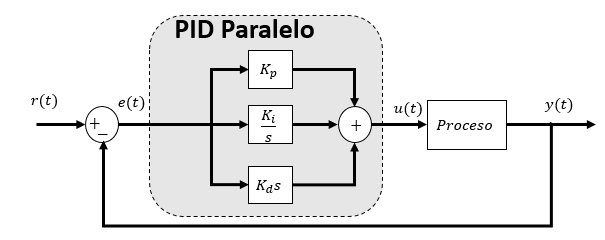
\includegraphics[width=0.85\textwidth]{imagenes/PID-esquema.png}\\[0.5ex]
    {\small \textbf{Figura \thefigure.} Esquema del funcionamiento de un PID.,  \cite{ImgEsquemaPID}.}
    \addcontentsline{lof}{figure}{\protect\numberline{\thefigure} Esquema de un PID}
 \end{center}

\vspace{0.3cm}

Si se define el error como:

\vspace{0.3cm}

\begin{equation}
e(t) = r(t) - y(t)
\end{equation}

\vspace{0.3cm}

donde $r(t)$ es la referencia deseada y $y(t)$ es la salida observada, entonces la señal de control generada por un PID puede expresarse como:

\vspace{0.4cm}

\begin{equation}
u(t) = K_p e(t) + K_i \int_{0}^{t} e(\tau) d\tau + K_d \frac{de(t)}{dt}
\end{equation}

\vspace{0.4cm}

Esta formulación combina tres contribuciones complementarias:

\begin{itemize}
    \item \textbf{Término proporcional ($K_p$).} Proporciona una respuesta inmediata en función del error actual. Si el objetivo está alejado de la referencia, la acción de control aumenta de forma proporcional para corregir esa desviación con rapidez.

    \item \textbf{Término integral ($K_i$).} Acumula el error a lo largo del tiempo. Su función principal es eliminar el error residual o estático, de modo que el sistema no se quede permanentemente cerca de la referencia sin llegar a alcanzarla completamente.

    \item \textbf{Término derivativo ($K_d$).} Actúa sobre la velocidad de cambio del error. Su efecto puede interpretarse como un amortiguamiento que anticipa la tendencia del sistema y ayuda a reducir oscilaciones o respuestas demasiado bruscas.
\end{itemize}

\vspace{0.4cm}

Desde un punto de vista funcional, el término proporcional aporta rapidez de reacción, el integral mejora la precisión final y el derivativo contribuye a suavizar la dinámica transitoria. La combinación adecuada de estas tres acciones permite construir un controlador que responda con suficiente rapidez sin comprometer la estabilidad del sistema.

\vspace{0.4cm}

Por estas razones, el PID sigue siendo una elección frecuente en plataformas embebidas que deben compartir recursos con módulos de percepción e inferencia en tiempo real. Frente a enfoques de control más complejos, ofrece una implementación ligera y una integración sencilla con los lazos internos del autopiloto, lo que explica su amplia presencia en aplicaciones de seguimiento visual de UAV.

\vspace{0.4cm}


\section{Estimación de Estado y Filtrado}

En sistemas de navegación visual, las observaciones extraídas por el detector suelen estar afectadas por ruido, retardos y pérdidas puntuales. Por ello, la literatura incorpora con frecuencia técnicas de estimación y filtrado que aportan coherencia temporal a la información perceptiva antes de utilizarla en el lazo de control. Entre las soluciones más extendidas destacan el filtro de Kalman y los métodos de suavizado recursivo, como el EMA, por su equilibrio entre coste computacional y capacidad para atenuar fluctuaciones de la señal.

\vspace{0.4cm}

\subsection{Origen y Evolución del Filtro de Kalman}

El filtro de Kalman es un método de estimación recursiva formulado por Rudolf E. Kalman en 1960 para inferir el estado de sistemas dinámicos lineales a partir de medidas afectadas por ruido. Su interés radica en que combina la predicción proporcionada por un modelo dinámico con la información de los sensores, obteniendo estimaciones más estables y consistentes que las medidas directas por sí solas \cite{kalman1960new, kalmanfilterNetES, wikipediaFiltroKalman}.

\vspace{0.4cm}

Con el tiempo, esta formulación se ha extendido a variantes no lineales, como el filtro de Kalman extendido (EKF), muy utilizadas en robótica móvil y aérea. En navegación visual con UAV, además, el filtrado suele integrarse con modelos dinámicos y estrategias predictivas para compensar retardos de percepción, suavizar detecciones y mantener la coherencia temporal del seguimiento.

\vspace{0.4cm}

\subsection{Fundamentos y Mecanismo Recursivo}

Desde un punto de vista operativo, el filtro funciona de manera recursiva y en tiempo real. En cada instante combina una etapa de predicción, basada en el modelo del sistema, con una etapa de actualización, en la que incorpora la nueva medida disponible. Esta estructura lo hace especialmente apropiado para plataformas embebidas, donde interesa limitar el coste computacional y no almacenar todo el historial de observaciones.

\vspace{0.4cm}

El sistema se representa mediante un modelo de espacio de estados:

\vspace{0.4cm}

\begin{equation}
\mathbf{x}_k = \mathbf{F}_k \mathbf{x}_{k-1} + \mathbf{B}_k \mathbf{u}_k + \mathbf{w}_k
\end{equation}

\vspace{0.4cm}

\begin{equation}
\mathbf{z}_k = \mathbf{H}_k \mathbf{x}_k + \mathbf{v}_k
\end{equation}

\vspace{0.4cm}

En estas ecuaciones, $\mathbf{x}_k$ representa el estado del sistema, $\mathbf{z}_k$ la observación disponible, $\mathbf{F}_k$ la dinámica del modelo y $\mathbf{H}_k$ la relación entre el estado y la medida. Los términos $\mathbf{w}_k$ y $\mathbf{v}_k$ modelan, respectivamente, el ruido del proceso y el ruido de medida.

\vspace{0.4cm}

\subsection{Aplicación en Persecución Visual y Alta Velocidad}

\vspace{0.4cm}

En sistemas de persecución visual, el filtrado de Kalman aporta continuidad temporal a las detecciones, atenúa el ruido de la medida y permite anticipar a corto plazo el movimiento del objetivo. Estas propiedades resultan especialmente relevantes cuando la información visual llega con retardos, presenta oclusiones parciales o debe combinarse con la dinámica del interceptor dentro del lazo de control.

\vspace{0.4cm}

En la literatura reciente, este tipo de estimación se integra con estrategias de navegación visual para fusionar la información procedente de la cámara con el modelo dinámico del vehículo, lo que contribuye a mantener trayectorias de seguimiento más estables y a reducir el efecto de fluctuaciones rápidas en la percepción. De este modo, el filtrado no sustituye al controlador, sino que mejora la calidad de la señal sobre la que este actúa.

\vspace{0.4cm}

Entre sus aportaciones más relevantes en este contexto pueden destacarse las siguientes:

\begin{itemize}
    \item \textbf{Continuidad temporal}: ayuda a mantener una estimación coherente del objetivo incluso ante pérdidas puntuales de detección.
    \item \textbf{Fusión entre modelo y medida}: combina la información visual con la predicción dinámica del sistema para reducir la sensibilidad al ruido.
    \item \textbf{Predicción a corto plazo}: facilita anticipar la evolución inmediata del blanco, algo especialmente útil en maniobras rápidas o agresivas.
\end{itemize}

\vspace{0.3cm}
\subsection{Filtro EMA}

El filtro EMA (\textit{Exponential Moving Average}), también denominado suavizado exponencial, es un método recursivo de suavizado utilizado para reducir las fluctuaciones rápidas de una señal sin necesidad de almacenar un gran número de muestras previas. Su interés principal reside en que requiere muy poca memoria y un coste computacional muy bajo, por lo que resulta especialmente adecuado para sistemas embebidos y aplicaciones de control en tiempo real \cite{industrialEma, wikipediaSuavizamientoExponencial, mciEma}.

\vspace{0.3cm}

Desde un punto de vista funcional, el EMA actúa como un filtro paso bajo: atenúa las variaciones de alta frecuencia asociadas al ruido y conserva la tendencia general de la señal. Por este motivo, se utiliza de forma habitual cuando se desea reducir la sensibilidad de una señal frente a pequeñas oscilaciones entre muestras consecutivas.

\vspace{0.3cm}

La formulación discreta del filtro EMA es la siguiente:

\vspace{0.3cm}

\begin{equation}
\hat{x}_k = \alpha x_k + (1-\alpha) \hat{x}_{k-1}
\end{equation}

\vspace{0.3cm}

donde $x_k$ representa la medida actual, $\hat{x}_k$ la salida filtrada y $\hat{x}_{k-1}$ el valor filtrado del instante anterior. El parámetro $\alpha$, con $0 < \alpha \leq 1$, determina el peso relativo entre la muestra nueva y el historial previo.

\vspace{0.3cm}

Esta expresión también puede escribirse como:

\vspace{0.3cm}

\begin{equation}
\hat{x}_k = \hat{x}_{k-1} + \alpha \left(x_k - \hat{x}_{k-1}\right)
\end{equation}

\vspace{0.3cm}

Esta segunda forma resulta útil para interpretar el funcionamiento del filtro: la nueva salida se obtiene corrigiendo el valor filtrado anterior en función de la diferencia entre la medida actual y la estimación previa. Si $\alpha$ toma valores pequeños, el suavizado es mayor y la respuesta del filtro es más lenta; si $\alpha$ se aproxima a 1, la salida sigue más de cerca la medida y el efecto de suavizado disminuye .

\vspace{0.3cm}

La Figura \ref{fig:ema-suavizado} ilustra este comportamiento sobre una señal ruidosa. En ella puede apreciarse cómo la salida filtrada atenúa las oscilaciones rápidas de la señal original y conserva su tendencia global.

\vspace{0.3cm}

\begin{center}
    \refstepcounter{figure}\label{fig:ema-suavizado}
    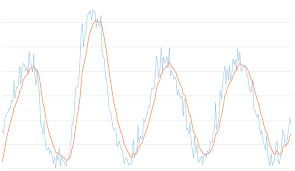
\includegraphics[width=0.58\textwidth]{imagenes/EMA.png}\\[0.5ex]
    {\small \textbf{Figura \thefigure.} Efecto del filtro EMA sobre una señal ruidosa. Fuente: \cite{mciEma}.}
    \addcontentsline{lof}{figure}{\protect\numberline{\thefigure} Efecto del filtro EMA sobre una señal ruidosa}
\end{center}

\vspace{0.3cm}

En consecuencia, el EMA constituye una técnica de suavizado sencilla, ligera y eficiente para señales discretas. Su bajo coste computacional y su formulación recursiva hacen que resulte especialmente útil en aplicaciones donde se requiere atenuar ruido de alta frecuencia sin introducir una complejidad elevada.

\section{Stack de Software y Hardware}

La sofisticación de los sistemas robóticos modernos, especialmente en el ámbito de las aeronaves no tripuladas que operan en entornos dinámicos, exige infraestructuras de software que permitan la ejecución paralela de procesos heterogéneos. En este contexto, resulta imperativo emplear marcos de trabajo que actúen como capas de abstracción o middleware, garantizando la interoperabilidad entre los diferentes módulos de percepción, planificación y control mediante intercambios de datos deterministas y eficientes. Estas plataformas aseguran una comunicación estandarizada entre procesos, facilitando la integración de algoritmos complejos de navegación autónoma.
\vspace{0.3cm}

\subsection{Intercambio de Datos en Robótica}

La coordinación de un sistema robótico distribuido requiere mecanismos capaces de mover datos entre procesos de forma ordenada, predecible y compatible con las necesidades temporales de cada módulo. En el caso de los UAVs, esta comunicación resulta especialmente crítica, ya que los bloques de percepción, estimación, planificación y control deben compartir información de manera continua para mantener una respuesta coherente durante el vuelo. Dentro de este marco se revisan tres alternativas representativas: DDS, MQTT y ROS, cada una con un enfoque distinto respecto a la organización de la red, la fiabilidad de los mensajes y su adecuación al control en tiempo real.

\vspace{0.3cm}

\subsubsection{DDS como Middleware Orientado a Datos}

Data Distribution Service (DDS) es un estándar definido por la \textit{Object Management Group} para sistemas distribuidos en los que la fiabilidad, el determinismo y la disponibilidad son requisitos de elevada importancia. Su diseño se apoya en una arquitectura descentralizada de publicación--suscripción, donde los productores y consumidores de información pueden descubrirse e intercambiar datos sin depender de un servidor central. Esta ausencia de un punto único de fallo mejora la tolerancia del sistema ante caídas de nodos o problemas puntuales de red, una propiedad especialmente valiosa en robótica móvil, vehículos autónomos y aplicaciones aeroespaciales.

\vspace{0.3cm}

Uno de los elementos más relevantes de DDS es la configuración de políticas de Calidad de Servicio (QoS). A través de ellas es posible ajustar parámetros como la latencia tolerada, la prioridad de los mensajes, la persistencia de la información y la fiabilidad de la entrega. Esta capacidad proporciona un control muy fino sobre el comportamiento temporal de la comunicación; sin embargo, también incrementa la complejidad de diseño. La selección incorrecta de las políticas QoS puede afectar al rendimiento global, por lo que su uso exige conocimiento técnico avanzado y una etapa de configuración cuidadosa.

\vspace{0.4cm}

\subsubsection{MQTT como Protocolo Ligero basado en Broker}

Message Queuing Telemetry Transport (MQTT) responde a una filosofía distinta. Se trata de un protocolo de mensajería ligero, concebido para redes con ancho de banda limitado y dispositivos con recursos computacionales reducidos, condiciones habituales en aplicaciones del Internet de las Cosas (IoT). A diferencia de los esquemas completamente descentralizados, MQTT introduce un \textit{broker} central que recibe los mensajes de los publicadores y los distribuye a los suscriptores correspondientes. Esta solución simplifica la topología de comunicación y facilita la integración de dispositivos heterogéneos.

\vspace{0.3cm}

Aunque MQTT permite trabajar con diferentes niveles de fiabilidad en la entrega de datos, su diseño no está orientado a cerrar lazos de control de baja latencia ni a sincronizar estados cinemáticos con la precisión temporal que requiere un UAV durante maniobras rápidas. Por este motivo, su uso en plataformas aéreas resulta más adecuado para tareas auxiliares, como telemetría, monitorización remota o transmisión de información no crítica. En cambio, para algoritmos de seguimiento visual o interceptación, donde el controlador debe reaccionar de forma continua ante cambios del objetivo, MQTT no ofrece las garantías temporales necesarias.

\vspace{0.4cm}
\subsection{Computación Distribuida Seleccionada}

La implementación del sistema de navegación autónoma para la interceptación de aeronaves no tripuladas requiere de una infraestructura de software capaz de gestionar procesos concurrentes con un alto grado de desacoplamiento. En este sentido, se ha seleccionado el paradigma de Robot Operating System (ROS) como el middleware central, integrando componentes críticos como MAVROS para la interfaz con el hardware de vuelo.

\vspace{0.4cm}

La decisión de emplear ROS frente a otras alternativas técnicas se sustenta en la versatilidad de su ecosistema y la modularidad de su arquitectura. Si bien soluciones como Data Distribution Service (DDS) ofrecen una gestión granular de las políticas de Calidad de Servicio (QoS) y un control estricto sobre el determinismo de la red, su implementación exige una especialización técnica que puede ralentizar las fases iniciales de prototipado. No obstante, la evolución hacia ROS 2 permite heredar las garantías de comunicación de DDS de forma subyacente, manteniendo una interfaz de programación de alto nivel que simplifica la integración de módulos complejos de percepción y control.

\vspace{0.4cm}

Esta arquitectura modular resulta fundamental para la naturaleza del proyecto, permitiendo que el nodo de proyección geométrica  pueda intercambiar información de forma eficiente con el bucle de control de guiado. A diferencia de protocolos como MQTT, que destacan por su ligereza en aplicaciones de telemetría y entornos de Internet de las Cosas (IoT), estos carecen de las capacidades necesarias para el control de actuadores en tiempo real y la sincronización de estados cinemáticos exigida en maniobras de persecución.

\vspace{0.4cm}

El ecosistema de ROS proporciona, además, una serie de bibliotecas  y herramientas de grabación de datos que agilizan el ciclo de validación experimental. Esta flexibilidad facilita el escalado del sistema, permitiendo la incorporación de nuevas capacidades de visión artificial o técnicas de filtrado estocástico sin comprometer la cohesión del diseño original.ROS se presenta como la opción más completa y robusta para
implementar un sistema de navegación vectorial distribuido, garantizando tanto la
eficiencia computacional como la cohesión arquitectónica del conjunto.


\subsubsection{ROS como Núcleo de la Arquitectura Modular}

En este proyecto, Robot Operating System (ROS) se adopta como el elemento vertebrador de la arquitectura distribuida, ya que permite coordinar procesos concurrentes sin imponer una estructura monolítica al sistema. Su función principal es actuar como middleware entre los algoritmos de alto nivel y los elementos asociados al vehículo, proporcionando una capa de abstracción que simplifica la comunicación, la supervisión y la integración de los distintos módulos. Esta capacidad resulta especialmente adecuada para navegación autónoma, donde percepción, estimación y control deben operar de forma simultánea y con dependencias bien definidas.

\vspace{0.3cm}

La organización interna de ROS se apoya en el concepto de nodo. Cada nodo representa una unidad lógica de ejecución encargada de una tarea específica, como procesar imágenes, calcular referencias de guiado, publicar estados del UAV o enviar comandos de control. Al tratarse de procesos independientes, pueden implementarse en distintos lenguajes de programación y evolucionar de manera separada, lo que incrementa la modularidad y facilita la depuración. El intercambio continuo de información entre ellos se realiza principalmente mediante tópicos, canales asíncronos que siguen un modelo de publicación--suscripción.

\vspace{0.3cm}

Junto a los tópicos, ROS ofrece mecanismos adicionales como servicios y acciones. Los servicios son apropiados para interacciones puntuales de tipo petición--respuesta, por ejemplo al consultar un estado concreto del vehículo o modificar una configuración. Las acciones, en cambio, están pensadas para procesos de mayor duración que requieren seguimiento, retroalimentación o cancelación. No obstante, la arquitectura desarrollada en este trabajo se apoya principalmente en tópicos, ya que los flujos de navegación visual, telemetría y control necesitan actualizaciones continuas y una comunicación más adecuada para operación en tiempo real.

\vspace{0.3cm}

\begin{center}
    \refstepcounter{figure}\label{fig:logo-Ros}
    
\includegraphics[width=0.58\textwidth]{imagenes/ROS.png}\\[0.5ex]
    {\small \textbf{Figura \thefigure.} Robot Operating System. Fuente: \cite{ROSLogo}.}
    \addcontentsline{lof}{figure}{\protect\numberline{\thefigure}Logo de ROS}
\end{center}

\vspace{0.3cm}

\subsubsection{Herramientas de Terminal para ROS}

La operación de ROS Noetic se apoya de forma habitual en la línea de comandos, tanto durante la puesta en marcha del sistema como en las fases de diagnóstico y depuración. En lugar de constituir comandos aislados, estas utilidades forman parte del flujo de trabajo necesario para iniciar la infraestructura de comunicación, lanzar nodos, consultar el estado de ejecución y comprobar el contenido de los mensajes intercambiados. La Tabla siguiente resume las instrucciones utilizadas con mayor frecuencia durante el desarrollo del proyecto.

\vspace{0.2cm}

\begin{longtable}{>{\raggedright\arraybackslash}p{0.36\textwidth}>{\raggedright\arraybackslash}p{0.56\textwidth}}
\textbf{Comando} & \textbf{Función dentro del flujo de trabajo} \\
\hline
\texttt{roscore} & Inicializa el maestro de ROS y los servicios básicos que permiten registrar nodos y habilitar el descubrimiento entre procesos. \\
\texttt{rosrun nombre\_paquete nombre\_nodo} & Ejecuta un nodo concreto incluido en un paquete previamente compilado, lo que resulta útil para pruebas individuales o depuración localizada. \\
\texttt{roslaunch nombre\_paquete archivo.launch} & Lanza de forma coordinada varios nodos, parámetros y configuraciones definidos en un archivo \texttt{.launch}, facilitando el arranque de escenarios más complejos. \\
\texttt{rosnode list} & Muestra los nodos activos registrados en el sistema y permite comprobar rápidamente qué procesos se encuentran en ejecución. \\
\texttt{rostopic list} & Enumera los tópicos disponibles en la sesión actual, ayudando a identificar los canales de comunicación publicados por los distintos módulos. \\
\texttt{rostopic echo nombre\_topico} & Visualiza en tiempo real los mensajes emitidos en un tópico específico, por lo que resulta esencial para verificar datos, formatos y posibles anomalías de comunicación. \\
\texttt{rosparam list} & Consulta el servidor de parámetros de ROS y permite revisar las variables de configuración cargadas durante la ejecución. \\
\end{longtable}


\subsubsection{MAVROS como Interfaz entre ROS y el Autopiloto}

MAVROS se emplea como la capa de interoperabilidad encargada de conectar la arquitectura ROS con MAVLink, protocolo de comunicación utilizado de forma habitual por autopilotos como PX4 y ArduPilot. Su función no se limita a transferir paquetes entre ambos entornos, sino que proporciona una traducción estructurada entre los mensajes, servicios y parámetros propios de ROS y las órdenes, estados y configuraciones que interpreta el controlador de vuelo. Gracias a esta abstracción, los módulos de percepción, estimación y control pueden operar sobre una interfaz uniforme sin depender de los detalles específicos del autopiloto utilizado.

\vspace{0.3cm}

Desde una perspectiva operativa, MAVROS establece un canal bidireccional entre los nodos desarrollados en ROS y el UAV, tanto en simulación como en una plataforma física. A través de esta conexión se recibe telemetría relativa a la posición, la velocidad, la actitud, el estado de vuelo y el modo de operación del vehículo. En sentido inverso, la misma interfaz permite enviar consignas de movimiento, comandos de misión y modificaciones de determinados parámetros. Esta comunicación continua resulta crítica en navegación autónoma, ya que el lazo de control necesita actualizarse con información reciente del vehículo y generar nuevas referencias durante la ejecución.

\vspace{0.3cm}

Dentro del sistema propuesto, MAVROS actúa como punto de enlace entre la navegación visual y el sistema de vuelo. Los algoritmos de seguimiento obtienen datos organizados para estimar el comportamiento del UAV, mientras que las correcciones calculadas por el controlador se remiten al autopiloto mediante una interfaz normalizada. Esta separación entre la lógica de alto nivel y el hardware concreto aumenta la reutilización del software, facilita el mantenimiento y reduce la dependencia de una configuración aérea específica.

\vspace{0.3cm}

Otro elemento clave es su integración con el sistema de transformaciones espaciales de ROS, gestionado mediante \texttt{tf}. Esta funcionalidad permite coordinar marcos de referencia como \texttt{map}, \texttt{odom} y \texttt{base\_link}, necesarios para interpretar la navegación del vehículo y relacionar las observaciones visuales con el movimiento del UAV. En escenarios con varios drones, la gestión de estos marcos requiere especial cuidado: si diferentes vehículos publican referencias con nombres comunes, pueden aparecer ambigüedades o solapamientos. Por ello, durante la integración fue necesario separar correctamente los datos publicados por cada UAV dentro del entorno de simulación.

\vspace{0.3cm}

En síntesis, MAVROS proporciona mucho más que una pasarela de comunicación con el autopiloto. Su incorporación permite desacoplar percepción, control y ejecución de vuelo dentro de una arquitectura distribuida, manteniendo al mismo tiempo modularidad, escalabilidad y portabilidad entre pruebas simuladas y aplicaciones sobre plataformas reales.

\subsubsection{Justificación de la Arquitectura Adoptada}

La selección de una arquitectura basada en ROS, MAVROS y MAVLink responde a criterios técnicos directamente relacionados con las necesidades del proyecto. En lugar de presentar estas ventajas como elementos aislados, la Tabla siguiente resume el papel que desempeña cada criterio dentro del diseño global del sistema.

\vspace{0.2cm}

\begin{longtable}{>{\raggedright\arraybackslash}p{0.25\textwidth}>{\raggedright\arraybackslash}p{0.67\textwidth}}
\textbf{Criterio} & \textbf{Aportación al sistema} \\
\hline
\textbf{Modularidad} & La división en nodos independientes permite desarrollar, probar y mantener cada bloque de forma progresiva, reduciendo el acoplamiento entre percepción, estimación y control. \\
\textbf{Escalabilidad} & La estructura distribuida facilita incorporar nuevos sensores, módulos de control o múltiples UAV sin modificar de manera sustancial la arquitectura base. \\
\textbf{Portabilidad} & El uso de estándares consolidados como ROS y MAVLink permite trasladar la lógica desarrollada desde simulación hacia plataformas reales con cambios limitados. \\
\textbf{Flexibilidad} & La integración de MAVROS permite trabajar con distintos autopilotos y configuraciones de vehículo bajo una interfaz homogénea, tanto en pruebas simuladas como en escenarios reales. \\
\end{longtable}

En conjunto, esta arquitectura satisface los requisitos técnicos del proyecto y, además, favorece un proceso de desarrollo más ordenado y sostenible. La combinación de ROS, MAVROS y herramientas de supervisión como RViz ofrece un entorno adecuado para diseñar, observar y validar el comportamiento del sistema. Asimismo, deja abierta la posibilidad de incorporar sensores más avanzados, nuevos algoritmos de percepción y estrategias cooperativas entre múltiples UAV en entornos distribuidos.



\subsection{Simulación}

La simulación constituye una etapa esencial en el desarrollo de sistemas robóticos autónomos y, en particular, en aplicaciones con vehículos aéreos no tripulados. Antes de trasladar un algoritmo a una plataforma física, es necesario disponer de un entorno controlado en el que sea posible estudiar el comportamiento dinámico del UAV, comprobar la estabilidad del controlador y analizar la respuesta del sistema ante perturbaciones, cambios de trayectoria o variaciones en las condiciones de operación. De este modo, el simulador actúa como un punto intermedio entre el diseño teórico y la validación experimental sobre hardware real.

\vspace{0.4cm}

Los simuladores tridimensionales permiten reproducir, con distintos grados de fidelidad, elementos propios del entorno físico, como la gravedad, las colisiones, la respuesta cinemática, determinadas aproximaciones aerodinámicas y la lectura de sensores virtuales. Esta capacidad facilita la repetición de ensayos bajo condiciones equivalentes, el ajuste iterativo de parámetros y la evaluación de la solución en escenarios que serían costosos o arriesgados de reproducir directamente con un dron real. Por ello, la simulación no solo reduce riesgos materiales, sino que también acelera la depuración de los módulos de percepción, comunicación y control.

\vspace{0.4cm}

La elección del simulador resulta especialmente relevante cuando la arquitectura se apoya en herramientas como ROS, MAVROS y autopilotos compatibles con MAVLink, ya que la utilidad del entorno no depende únicamente de su calidad visual o de su motor físico, sino también de su capacidad para integrarse de forma estable con el resto del sistema. En este contexto, se han considerado distintas alternativas utilizadas habitualmente en robótica y navegación autónoma, entre las que destacan AirSim, Webots y Gazebo.



\subsubsection{AirSim}

AirSim es un simulador orientado a vehículos autónomos, desarrollado por Microsoft sobre el motor gráfico Unreal Engine. Su principal ventaja reside en la elevada calidad visual de los escenarios y en la posibilidad de emular sensores habituales en plataformas aéreas, como cámaras RGB, LIDAR, IMU o GPS. Estas características lo convierten en una herramienta atractiva para investigaciones centradas en visión por computador, aprendizaje por refuerzo o navegación basada principalmente en percepción.

\vspace{0.4cm}

Sin embargo, en el marco de este proyecto presenta algunas limitaciones relevantes. Aunque puede conectarse con ROS, su integración no resulta tan directa como en otras plataformas más extendidas dentro de la robótica experimental, y la comunicación con autopilotos como PX4 o ArduPilot suele requerir una configuración adicional. A ello se añade la carga computacional asociada a Unreal Engine, que puede dificultar la ejecución simultánea de varios UAV y ralentizar el ciclo de pruebas cuando se pretende evaluar una arquitectura distribuida completa.

\subsubsection{Webots}

Webots, desarrollado por Cyberbotics, es una solución de código abierto ampliamente empleada en docencia e investigación. Ofrece una interfaz accesible, compatibilidad con distintos lenguajes de programación y soporte para una variedad amplia de sensores, actuadores y modelos robóticos. Además, dispone de integración con ROS, especialmente en entornos vinculados con ROS 2, por lo que constituye una plataforma versátil para el prototipado y la validación de aplicaciones de robótica general.

\vspace{0.4cm}

No obstante, su idoneidad disminuye cuando el objetivo es reproducir un sistema UAV completo gobernado por autopilotos reales. La conexión con plataformas como PX4 o ArduPilot no alcanza el mismo grado de madurez que en otros entornos más utilizados para simulación aérea con SITL, y su motor físico, aunque suficiente para numerosos casos, puede resultar menos adecuado para analizar maniobras exigentes, control fino de trayectoria o escenarios multivehículo con mayor realismo dinámico.

\subsubsection{Gazebo}

Gazebo se ha consolidado como uno de los simuladores más utilizados en robótica por su equilibrio entre realismo físico, flexibilidad y facilidad de integración con el ecosistema ROS. Su arquitectura basada en plugins, la posibilidad de construir mundos modificables y la compatibilidad con múltiples sensores y modelos robóticos permiten ensayar algoritmos de navegación, percepción y control en condiciones reproducibles.

\vspace{0.4cm}

En proyectos centrados en UAV, esta combinación de fidelidad e interoperabilidad resulta especialmente valiosa. Gazebo puede conectarse con ROS mediante paquetes específicos y, a través de MAVROS y MAVLink, enlazarse con autopilotos como PX4 o ArduPilot. De este modo, los nodos de control pueden intercambiar consignas y telemetría con el vehículo simulado siguiendo una estructura cercana a la que se emplearía en una plataforma real, lo que facilita la automatización de experimentos y la reproducción de escenarios con varios agentes.

\subsection{Simulador Seleccionado}

Atendiendo a las necesidades del proyecto, Gazebo ha sido el simulador seleccionado para el desarrollo y la validación del sistema de navegación propuesto. La decisión se basa en su amplia implantación en robótica, su integración natural con ROS y su capacidad para representar entornos físicos configurables sin separar la simulación del resto de la arquitectura software. Mediante paquetes como \texttt{gazebo\_ros} y \texttt{gazebo\_plugins}, el simulador permite incorporar modelos de sensores, publicar información en tópicos ROS y conectar la dinámica del entorno con los nodos encargados de la percepción y el control.

\vspace{0.3cm}

Uno de los aspectos más relevantes de esta elección es la integración con MAVROS, que permite enlazar la simulación con un autopiloto virtual basado en PX4 o ArduPilot a través del protocolo MAVLink. Así, las consignas generadas por los nodos de control se envían al UAV virtual de forma análoga a como se enviarían a un dron real, mientras que la telemetría producida por el autopiloto se redistribuye al resto de módulos ROS. Esta continuidad entre percepción, control, autopiloto y simulación resulta fundamental para validar el comportamiento global del sistema sin abandonar un entorno seguro, repetible y controlado.


\begin{center}
\refstepcounter{figure}\label{fig:Gazebo-camera}
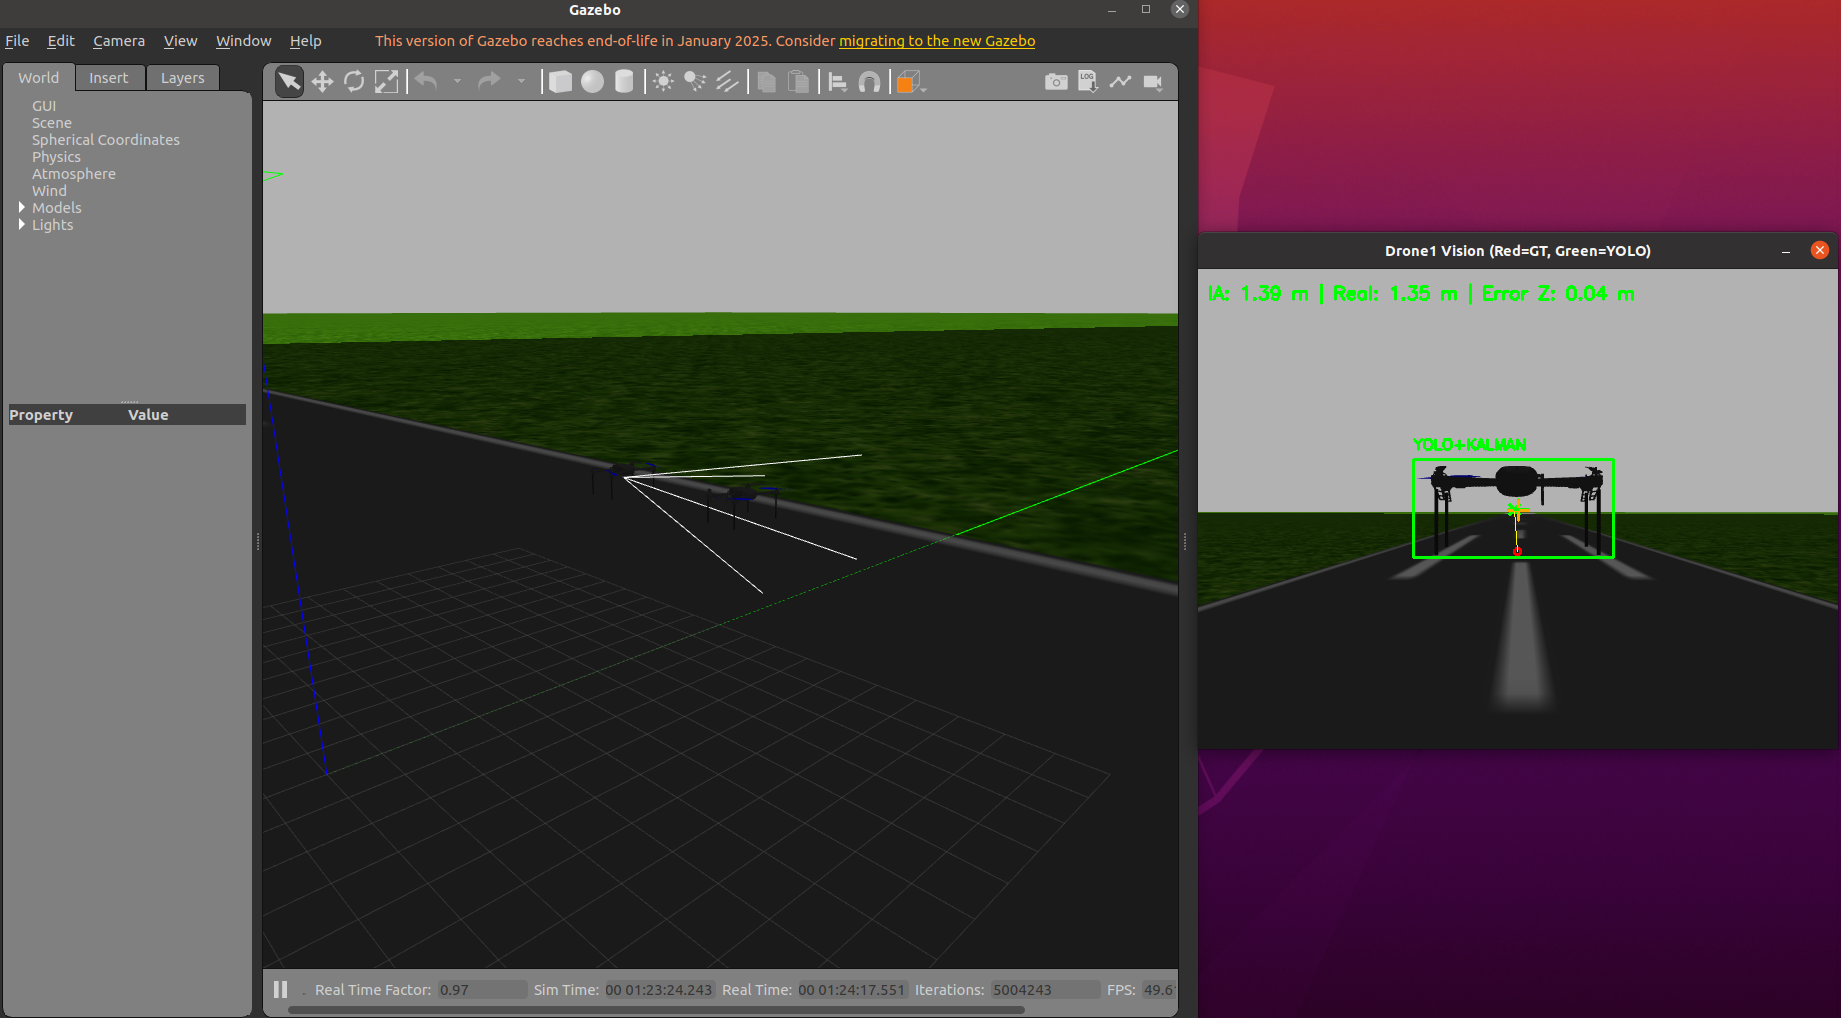
\includegraphics[width=0.8\textwidth]{imagenes/Gazebo+camera_2.png}\\[0.5ex]
{\small \textbf{Figura \thefigure.} Uso de Gazebo con la camara. (Imagen de Elaboración Propia).}
\addcontentsline{lof}{figure}{\protect\numberline{\thefigure} Uso de Gazebo con la camara. (Imagen de Elaboración Propia)}
\end{center}


\vspace{0.3cm}

En la práctica, Gazebo ha desempeñado un papel fundamental durante las fases de diseño, prueba y ajuste del sistema, ya que ha permitido analizar la respuesta del UAV ante cambios de trayectoria, maniobras de seguimiento y variaciones del entorno de forma repetible y sin riesgo para la plataforma física. Además, su compatibilidad con ROS, MAVROS, PX4 y ArduPilot facilita que los resultados obtenidos en simulación puedan trasladarse posteriormente a una configuración real con cambios limitados en la arquitectura de comunicación.

\vspace{0.3cm}

Aun así, la simulación no elimina por completo el denominado \textit{sim2real gap}, es decir, las diferencias inevitables entre el entorno virtual y el comportamiento real del vehículo. Factores como las latencias, el ruido sensorial, las condiciones aerodinámicas o ciertas dinámicas no modeladas obligan a interpretar Gazebo como una etapa crítica de validación previa, pero no como un sustituto definitivo de las pruebas experimentales sobre hardware real.
